%%-----------------------------------------------------------------------------
%%
%%                                   Sean Mauch
%%                       California Institute of Technology
%%                        @ 1995-2004 No Rights Reserved
%%
%%-----------------------------------------------------------------------------

\flushbottom




%%============================================================================
%%============================================================================
\chapter{Complex Numbers}



I'm sorry.  You have reached an imaginary number.  Please rotate your phone
$90$ degrees and dial again.

\begin{flushright}
  -Message on answering machine of Cathy Vargas.
\end{flushright}








%%=============================================================================
\section{Complex Numbers}
\index{complex numbers}






\paragraph{Shortcomings of real numbers.}
When you started algebra, you learned that the quadratic equation:
$x^2 + 2 a x + b = 0$ has either two, one or no solutions.  For example:
\begin{itemize}
\item
  $x^2 - 3 x + 2 = 0$ has the two solutions $x = 1$ and $x = 2$.
\item
  For $x^2 - 2 x + 1 = 0$, $x = 1$ is a solution of multiplicity two.
\item
  $x^2 + 1 = 0$ has no solutions.
\end{itemize}
This is a little unsatisfactory.  
We can formally solve the general quadratic equation.
\begin{gather*}
  x^2 + 2 a x + b = 0 
  \\
  (x + a)^2 = a^2 - b 
  \\
  x = -a \pm \sqrt{a^2 - b}
\end{gather*}
However, the solutions are defined only when the discriminant $a^2 -
b$ is non-negative.  This is because the square root function $\sqrt{x}$
is a bijection from $\mathbb{R}^{0+}$ to $\mathbb{R}^{0+}$.  (See
Figure~\ref{figure fcv number yesqrtx}.)
\begin{figure}[h!]
  \begin{center}
    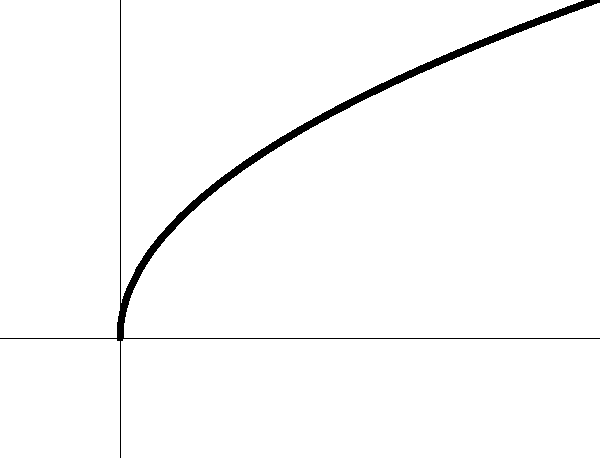
\includegraphics[width=0.3\textwidth]{fcv/number/yesqrtx}
  \end{center}
  \caption{The square root function.}
  \label{figure fcv number yesqrtx}
\end{figure}




\paragraph{A new mathematical constant.}
We cannot solve $x^2 = -1$ because the square root of $-1$ is not defined.  To
overcome this apparent shortcoming of the real number system, we
create a new symbolic constant $\sqrt{-1}$.  In performing arithmetic,
we will treat $\sqrt{-1}$ as we would a real constant like $\pi$ or a 
formal variable like $x$, i.e. $\sqrt{-1} + \sqrt{-1} = 2 \sqrt{-1}$.
This constant has the property:
$\left( \sqrt{-1} \right)^2 = -1$.  Now we can express the solutions
of $x^2 = -1$ as $x = \sqrt{-1}$ and $x = - \sqrt{-1}$.  These satisfy
the equation since $\left( \sqrt{-1} \right)^2 = -1$ and 
$\left( - \sqrt{-1} \right)^2 = (-1)^2 \left( \sqrt{-1} \right)^2 = -1$.
Note that we can express the square root of any negative real number in 
terms of $\sqrt{-1}$: $\sqrt{-r} = \sqrt{-1} \sqrt{r}$ for $r \geq 0$.  



\paragraph{Euler's notation.}
Euler introduced the notation of using the letter $i$ to denote $\sqrt{-1}$.
\index{i!Euler's notation}
\index{Euler's notation!i}
We will use the symbol $\imath$, an $i$ without a dot, to denote 
$\sqrt{-1}$.  This helps us distinguish it from $i$ used as a variable or 
index.%
\footnote{
  Electrical engineering types prefer to use $\jmath$ or $j$ to denote
  $\sqrt{-1}$.
  \index{j electrical engineering}
  }
We call any number of the form $\imath b$, 
$b \in \mathbb{R}$, a \textit{pure imaginary number}.%
\footnote{
  ``Imaginary'' is an unfortunate term.  Real numbers are 
  artificial; constructs of the mind.  Real numbers are no more real than
  imaginary numbers.
  }
\index{pure imaginary number}
\index{imaginary number}
Let $a$ and $b$ be real numbers.  The product of a real number and an 
imaginary number is an imaginary number: $(a)(\imath b) = \imath (a b)$.
The product of two imaginary numbers is a real number: 
$(\imath a)(\imath b) = - a b$.  However the sum of a real number and an 
imaginary number $a + \imath b$ is neither real nor imaginary.
We call numbers of the form $a + \imath b$ \textit{complex numbers}.%
\footnote{
  Here complex means ``composed of two or more parts'', not
  ``hard to separate, analyze, or solve''.  Those who disagree have a 
  complex number complex.
  }
\index{complex number}


\paragraph{The quadratic.}
Now we return to the quadratic with real coefficients, 
$x^2 + 2 a x + b = 0$.  It has the solutions
$x = -a \pm \sqrt{a^2 - b}$.  The solutions are real-valued
only if $a^2 - b \geq 0$.  If not, then we can define solutions as 
complex numbers.  
If the discriminant is negative, we write
$x = -a \pm \imath \sqrt{b - a^2}$.
Thus every quadratic polynomial with real coefficients has exactly 
two solutions, counting multiplicities.  
The fundamental theorem of algebra states that an $n^{\mathrm{th}}$
degree polynomial with complex coefficients has $n$, not necessarily
distinct, complex roots.  We will prove this result later using the 
theory of functions of a complex variable.





\paragraph{Component operations.}
Consider the complex number $z = x + \imath y$, $(x,y \in \mathbb{R})$.  
The \textit{real part} of $z$ is 
\index{real part}
$\Re(z) = x$; the \textit{imaginary part} of $z$ is $\Im(z) = y$.
\index{imaginary part}
Two complex numbers, $z = x + \imath y$ and $\zeta = \xi + \imath \psi$, are equal
if and only if $x = \xi$ and $y = \psi$.  The \textit{complex conjugate}%
\footnote{
  Conjugate: having features in common but opposite or inverse in 
  some particular.
  }
\index{complex conjugate}
of $z = x + \imath y$ is $\overline{z} \equiv x - \imath y$.  The notation 
$z^* \equiv x - \imath y$ is also used.


\paragraph{A little arithmetic.}
Consider two complex numbers: $z = x + \imath y$, $\zeta = \xi + \imath \psi$.
It is easy to express the sum or difference as a complex number.
\[
z + \zeta = (x + \xi) + \imath(y + \psi), \quad
z - \zeta = (x - \xi) + \imath(y - \psi)
\]
It is also easy to form the product.
\[
z \zeta = (x + \imath y)(\xi + \imath \psi)
= x \xi + \imath x \psi + \imath y \xi + \imath^2 y \psi
= (x \xi - y \psi) + \imath(x \psi + y \xi)
\]
The quotient is a bit more difficult.  (Assume that $\zeta$ is nonzero.)  How do
we express $z / \zeta = (x + \imath y) / (\xi + \imath \psi)$ as the sum of a real
number and an imaginary number?  The trick is to multiply the numerator and
denominator by the complex conjugate of $\zeta$.
\[
\frac{z}{\zeta} 
= \frac{x + \imath y}{\xi + \imath \psi}
= \frac{x + \imath y}{\xi + \imath \psi} \frac{\xi - \imath \psi}{\xi - \imath \psi}
= \frac{x \xi - \imath x \psi - \imath y \xi - \imath^2 y \psi}
{\xi^2 - \imath \xi \psi + \imath \psi \xi - \imath^2 \psi^2}
= \frac{(x \xi + y \psi) - \imath (x \psi + y \xi)}
{\xi^2 + \psi^2}
= \frac{(x \xi + y \psi)}{\xi^2 + \psi^2} - \imath \frac{x \psi + y \xi}{\xi^2 + \psi^2}
\]
Now we recognize it as a complex number.


\paragraph{Field properties.}
The set of complex numbers $\mathbb{C}$ form a field.  That essentially
means that we can do arithmetic with complex numbers.
When performing arithmetic, we simply treat $\imath$ as a symbolic 
constant with the property that $\imath^2 = -1$.
The field of complex numbers satisfy the following list of properties.
Each one is easy to verify; some are proved below.
(Let $z, \zeta, \omega \in \mathbb{C}$.)
\begin{enumerate}
\item
  Closure under addition and multiplication.
  \begin{align*}
    z + \zeta &= \left( x + \imath y \right) + \left(\xi + \imath \psi \right) 
    \\
    &= \left( x + \xi \right) + \imath \left( y + \psi \right) \in \mathbb{C} 
    \\
    z \zeta &= \left( x + \imath y \right) \left( \xi + \imath \psi \right) 
    \\
    &= x \xi + \imath x \psi + \imath y \xi + \imath^2 y \psi
    \\
    &= \left( x \xi - y \psi \right) 
    + \imath \left( x \psi + \xi y \right) \in \mathbb{C}
  \end{align*}
\item
  Commutativity of addition and multiplication.  $z + \zeta = \zeta + z$.
  $z \zeta = \zeta z$.
\item
  Associativity of addition and multiplication.  
  $\left( z + \zeta \right) + \omega = z + \left( \zeta  + \omega \right)$.
  $\left( z \zeta \right) \omega = z \left( \zeta \omega \right)$.
\item
  Distributive law.  $z \left( \zeta + \omega \right) = z \zeta + z \omega$.
\item
  Identity with respect to addition and multiplication.  Zero is the 
  additive identity element, $z + 0 = z$; unity is the muliplicative
  identity element, $z (1) = z$.
\item
  Inverse with respect to addition.
  $z + (-z)= (x + \imath y) + (- x - \imath y) = (x - x) + \imath(y - y) = 0$.
\item
  Inverse with respect to multiplication for nonzero numbers.
  $z z^{-1} = 1$, where 
  \[
  z^{-1} 
  = \frac{1}{z} 
  = \frac{1}{x + \imath y} 
  = \frac{1}{x + \imath y} \frac{x - \imath y}{x - \imath y} 
  = \frac{x - \imath y}{x^2 + y^2}
  = \frac{x}{x^2 + y^2} - \imath \frac{y}{x^2 + y^2}
  \]
\end{enumerate}





\paragraph{Properties of the complex conjugate.} 
\index{complex conjugate}
Using the field properties of complex numbers, we can derive 
the following properties of the complex conjugate, 
$\overline{z} = x - \imath y$.
\begin{enumerate}
\item
  $\displaystyle \overline{\left( \overline{z} \right)} = z$, 
\item
  $\displaystyle \overline{z + \zeta} = \overline{z} + \overline{\zeta}$, 
\item
  $\displaystyle \overline{z \zeta} = \overline{z} \overline{\zeta}$, 
\item
  $\displaystyle \overline{ \left( \frac{z}{\zeta} \right) } 
  = \frac{ \left( \overline{z} \right) }{ \left( \overline{\zeta} \right) }$. 
\end{enumerate}











%%=============================================================================
\section{The Complex Plane}





\paragraph{Complex plane.}
We can denote a complex number $z = x + \imath y$ as an ordered pair of real
numbers $(x,y)$.  Thus we can represent a complex number as a point in 
$\mathbb{R}^2$ where the first component is the real part and the second 
component is the imaginary part of $z$.  This is called the 
\textit{complex plane} 
\index{complex plane}
or the \textit{Argand diagram}.  (See Figure~\ref{complexplane}.)
\index{Argand diagram}
A complex number written as $z = x + \imath y$ is said to be in 
\textit{Cartesian form}, or \textit{$a + \imath b$ form}.
\index{Cartesian form}
\index{a + i b form}

\begin{figure}[h!]
  \begin{center}
    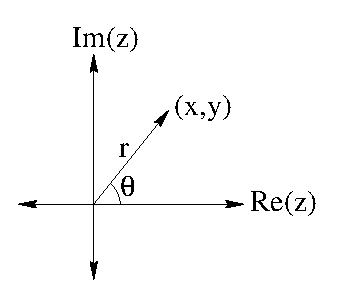
\includegraphics[width=0.25\textwidth]{fcv/number/comp_pln}
  \end{center}
  \caption{The complex plane.}
  \label{complexplane}
\end{figure}


Recall that there are two ways of describing a point in the complex plane: an
ordered pair of coordinates $(x, y)$ that give the horizontal and
vertical offset from the origin or the distance $r$ from the origin
and the angle $\theta$ from the positive horizontal axis.  The angle $\theta$
is not unique.  It is only determined up to an additive integer
multiple of $2 \pi$.




\paragraph{Modulus.}
The \textit{magnitude} or \textit{modulus} of a complex number is the 
\index{magnitude}
\index{modulus}
\index{complex number!magnitude}
\index{complex number!modulus}
distance of the point from the origin.  It is defined 
as $|z| = |x + \imath y| = \sqrt{x^2 + y^2}$.  Note that 
$z \overline{z} = (x + \imath y)(x - \imath y) = x^2 + y^2 = |z|^2$.
The modulus has the following properties.
\begin{enumerate}
\item
  $\displaystyle \left|z \zeta \right| = \left|z \right| \left|\zeta \right|$
\item
  $\displaystyle \left| \frac{z}{\zeta} \right| = \frac{ \left|z \right|}
  { \left|\zeta \right|}$ for $\zeta \neq 0$.
\item
  $\displaystyle \left|z + \zeta \right| \leq \left|z \right| + \left|\zeta \right|$
\item
  $\displaystyle \left|z + \zeta \right| 
  \geq \left|\left|z \right| - \left|\zeta \right| \right|$
\end{enumerate}
We could prove the first two properties by expanding in $x + \imath y$ form, 
but it would be fairly messy.  The proofs will become simple after polar 
form has been introduced.  The second two properties
follow from the triangle inequalities in geometry.  This will become apparent
after the relationship between complex numbers and vectors is introduced.
One can show that
\[
\left|z_1 z_2 \cdots z_n \right| 
= \left|z_1 \right| \left|z_2 \right| \cdots \left|z_n \right|
\]
and
\[
\left|z_1 + z_2 + \cdots + z_n \right| 
\leq \left|z_1 \right| + \left|z_2 \right| + \cdots + \left|z_n \right|
\]
with proof by induction.



\paragraph{Argument.}
The \textit{argument} of a complex number is the angle that the vector with
\index{argument!of a complex number}
tail at the origin and head at $z = x + \imath y$ makes with the positive 
$x$-axis.  The argument is denoted $\arg(z)$. 
Note that the argument is defined for all nonzero numbers and 
is only determined up to an additive integer multiple
of $2 \pi$.  That is, the argument of a complex number is the set of values:
$\{ \theta + 2 \pi n \mid n \in \mathbb{Z}\}$.  The \textit{principal argument}
\index{principal argument}
of a complex number is that angle in the set $\arg(z)$ which lies in the
range $(-\pi,\pi]$.  The principal argument is denoted $\Arg(z)$.
We prove the following identities in Exercise~\ref{exercise argument identities}.
\begin{gather*}
  \arg(z \zeta) = \arg(z) + \arg(\zeta) \\
  \Arg(z \zeta) \neq \Arg(z) + \Arg(\zeta) \\
  \arg\left( z^2 \right) = \arg(z) + \arg(z) \neq 2 \arg(z)
\end{gather*}



\begin{Example}
  Consider the equation $|z - 1 - \imath| = 2$.  The set of points satisfying 
  this equation
  is a circle of radius 2 and center at $1 + \imath$ in the complex plane.  You
  can see this by noting that $|z - 1 - \imath|$ is the distance from the point
  $(1,1)$.
  (See Figure~\ref{circ211}.)
  \begin{figure}[h!]
    \begin{center}
      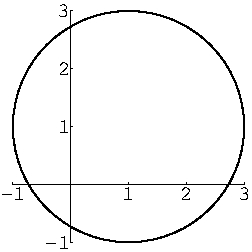
\includegraphics[width=0.3\textwidth]{fcv/number/circ211}
    \end{center}
    \caption{The solution is a circle.}
    \label{circ211}
  \end{figure}

  Another way to derive this is to substitute $z = x + \imath y$ 
  into the equation.
  \begin{gather*}
    |x + \imath y - 1 - \imath| = 2 
    \\
    \sqrt{(x-1)^2 + (y-1)^2} = 2 
    \\
    (x-1)^2 + (y-1)^2 = 4
  \end{gather*}
  This is the analytic geometry equation for a circle of radius 2 
  centered about $(1,1)$.  
\end{Example}







\begin{Example}
  Consider the curve described by 
  \[
  |z| + |z - 2| = 4.
  \]
  Note that $|z|$ is the distance from the origin in the complex plane and
  $|z - 2|$ is the distance from $z = 2$.  The equation is
  \[ 
  (\mathrm{distance from}\ (0,0)) + (\mathrm{distance from}\ (2,0)) = 4. 
  \]
  From geometry, we know that this is an ellipse with foci at $(0,0)$
  and $(2,0)$, major axis 2, and minor axis $\sqrt{3}$. 
  (See Figure~\ref{ellipse}.)
  \begin{figure}[h!]
    \begin{center}
      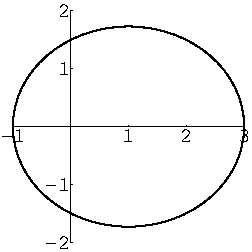
\includegraphics[width=0.3\textwidth]{fcv/number/ellipse}
    \end{center}
    \caption{The solution is an ellipse.}
    \label{ellipse}
  \end{figure}

  We can use the substitution $z = x + \imath y$ to get the equation in algebraic 
  form.
  \begin{gather*}
    |z| + |z - 2| = 4 
    \\
    |x + \imath y| + |x + \imath y - 2| = 4 
    \\
    \sqrt{x^2 + y^2} + \sqrt{(x - 2)^2 + y^2} = 4 
    \\
    x^2 + y^2 = 16 - 8 \sqrt{ (x - 2)^2 + y^2 } + x^2 - 4 x + 4 + y^2 
    \\
    x - 5 = -2 \sqrt{ (x - 2)^2 + y^2 } 
    \\
    x^2 - 10 x + 25 = 4 x^2 - 16 x + 16 + 4 y^2 
    \\
    \frac{1}{4} (x - 1)^2 + \frac{1}{3} y^2 = 1
  \end{gather*}
  Thus we have the standard form for an equation describing an ellipse.
\end{Example}






%%=============================================================================
\section{Polar Form}





\paragraph{Polar form.}
A complex number written in Cartesian form, $z = x + \imath y$,
can be converted \textit{polar form},
\index{polar form}
$z = r (\cos \theta + \imath \sin \theta)$, using trigonometry.
Here $r = |z|$ is the modulus and $\theta = \arctan(x,y)$ is 
the argument of $z$.  The argument is the angle between the $x$ axis and
the vector with its head at $(x,y)$.  (See Figure~\ref{polarfrm}.)
Note that $\theta$ is not unique.  If $z = r (\cos \theta + \imath \sin \theta)$ 
then $z = r (\cos (\theta + 2 n \pi) + \imath \sin (\theta + 2 n \pi) )$ for any
$n \in \mathbb{Z}$.

\begin{figure}[h!]
  \begin{center}
    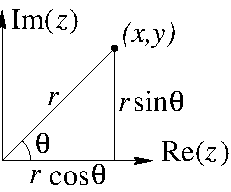
\includegraphics[width=0.2\textwidth]{fcv/number/polarfrm}
  \end{center}
  \caption{Polar form.}
  \label{polarfrm}
\end{figure}




\paragraph{The arctangent.}
Note that $\arctan(x,y)$ is not the same thing as the old arctangent that
you learned about in trigonometry
$\arctan(x,y)$ is sensitive to the quadrant of the point $(x,y)$, while
$\arctan\left(\frac{y}{x} \right)$ is not.
For example,
\[
\arctan(1,1) = \frac{\pi}{4} + 2 n \pi \quad \mathrm{and} \quad
\arctan(-1,-1) = \frac{-3 \pi}{4} + 2 n \pi,
\]
whereas
\[
\arctan \left( \frac{-1}{-1} \right) = \arctan \left(\frac{1}{1} \right)
= \arctan(1).
\]




\paragraph{Euler's formula.}
\textit{Euler's formula}, $\e^{\imath \theta} = \cos \theta + \imath \sin \theta$,%
\footnote{
  See Exercise~\ref{exercise eulers formula} for justification of 
  Euler's formula.
  }
\index{Euler's formula}
allows us to write the polar form more compactly.  Expressing 
the polar form in terms of the exponential function of imaginary argument
makes arithmetic with complex numbers much more convenient.
\[
z = r (\cos \theta + \imath \sin \theta) = r \e^{\imath \theta}
\]
The exponential of an imaginary argument has all the nice properties that
we know from studying functions of a real variable, like
$\e^{\imath a} \e^{\imath b} = \e^{\imath(a + b)}$.  Later on we will 
introduce the exponential of a complex number.

Using Euler's Formula, we can express the cosine and sine in terms of the
exponential.
\begin{gather*}
  \frac{\e^{\imath \theta} + \e^{-\imath \theta}}{2}
  = \frac{(\cos(\theta) + \imath \sin(\theta)) + (\cos(-\theta) + \imath \sin(-\theta))}{2}
  = \cos(\theta)
  \\
  \frac{\e^{\imath \theta} - \e^{-\imath \theta}}{\imath 2}
  = \frac{(\cos(\theta) + \imath \sin(\theta)) - (\cos(-\theta) + \imath \sin(-\theta))}{\imath 2}
  = \sin(\theta)
\end{gather*}






\paragraph{Arithmetic with complex numbers.}
Note that it is convenient to add complex numbers in Cartesian form.
\[
z + \zeta
= \left( x + \imath y \right) + \left( \xi + \imath \psi \right) 
= \left( x + \xi \right) + \imath \left( y + \psi \right)
\]
However, it is difficult to multiply or divide them in Cartesian form.
\begin{gather*}
  z \zeta
  = \left( x + \imath y \right)  \left( \xi + \imath \psi \right) 
  = \left( x \xi - y \psi \right) + \imath \left( x \psi + \xi y \right)
  \\
  \frac{z}{\zeta}
  = \frac{x + \imath y}{\xi + \imath \psi}
  = \frac{\left( x + \imath y \right)  \left( \xi - \imath \psi \right)}
  {\left( \xi + \imath \psi \right)  \left( \xi - \imath \psi \right)}
  = \frac{x \xi + y \psi}{\xi^2 + \psi^2}
  + \imath \frac{\xi y - x \psi}{\xi^2 + \psi^2}
\end{gather*}
On the other hand, it is difficult to add complex numbers in polar form.
\begin{align*}
  z + \zeta
  &= r \e^{\imath \theta} + \rho \e^{\imath \phi}
  \\
  &= r \left( \cos \theta + \imath \sin \theta \right) 
  + \rho \left( \cos \phi + \imath \sin \phi \right) 
  \\
  &= r \cos \theta + \rho \cos \phi
  + \imath \left( r \sin \theta + \rho \sin \phi \right) 
  \\
  &= \sqrt{ \left( r \cos \theta + \rho \cos \phi \right)^2
    + \left( r \sin \theta + \rho \sin \phi \right)^2 } 
  \\
  &\qquad \times \e^{\imath \arctan \left( 
      r \cos \theta + \rho \cos \phi, 
      r \sin \theta + \rho \sin \phi \right)} 
  \\
  &= \sqrt{ r^2 + \rho^2 + 2 \cos \left( \theta - \phi \right) }
  \e^{\imath \arctan \left( 
      r \cos \theta + \rho \cos \phi,
      r \sin \theta + \rho \sin \phi \right)} 
\end{align*}
However, it is convenient to multiply and divide them in polar form.
\begin{gather*}
  z \zeta
  = r \e^{\imath \theta} \rho \e^{\imath \phi} = r \rho \e^{\imath \left( \theta + \phi \right)}
  \\
  \frac{z}{\zeta}
  = \frac{r \e^{\imath \theta}}{\rho \e^{\imath \phi}}
  = \frac{r}{\rho} \e^{\imath \left( \theta - \phi \right)}
\end{gather*}
Keeping this in mind will make working with complex numbers a shade or 
two less grungy.






\begin{Result}
  \label{cartesian_and_polar_form}
  Euler's formula is 
  \[
  \e^{\imath \theta} = \cos \theta + \imath \sin \theta.
  \]
  We can write the cosine and sine in terms of the exponential.
  \[
  \cos(\theta) = \frac{\e^{\imath \theta} + \e^{-\imath \theta}}{2}, 
  \qquad
  \sin(\theta) = \frac{\e^{\imath \theta} - \e^{-\imath \theta}}{\imath 2}
  \]
  To change between Cartesian and polar form, use the identities
  \begin{align*}
    r \e^{\imath \theta} &= r \cos \theta + \imath r \sin \theta, 
    \\
    x + \imath y &= \sqrt{x^2 + y^2} \e^{\imath \arctan(x,y)}.
  \end{align*}
  Cartesian form is convenient for addition.  Polar form is convenient 
  for multiplication and division.
\end{Result}







\begin{Example}
  We write $5 + \imath 7$ in polar form.
  \[
  5 + \imath 7 = \sqrt{74} \e^{\imath \arctan(5,7) }
  \]
  We write $2 \e^{\imath \pi / 6}$ in Cartesian form.
  \begin{align*}
    2 \e^{\imath \pi / 6} 
    &= 2 \cos \left( \frac{\pi}{6} \right) 
    + 2 \imath \sin \left( \frac{\pi}{6} \right) 
    \\
    &= \sqrt{3} + \imath
  \end{align*}
\end{Example}








\begin{Example}
  We will prove the trigonometric identity
  \[
  \cos^4 \theta = \frac{1}{8} \cos(4 \theta) +
  \frac{1}{2} \cos(2 \theta) + \frac{3}{8}.
  \]
  We start by writing the cosine in terms of the exponential.
  \begin{align*}
    \cos^4 \theta   
    &=  \left(\frac{\e^{\imath \theta} + \e^{-\imath \theta}}{2}\right)^4 
    \\
    &=  \frac{1}{16} \left( \e^{\imath 4 \theta} + 4 \e^{\imath 2 \theta} + 6 +
    4 \e^{-\imath 2 \theta} + \e^{-\imath 4 \theta} \right) 
    \\
    &=  \frac{1}{8} \left( \frac{\e^{\imath 4 \theta} + \e^{-\imath 4 \theta}}{2} \right) +
    \frac{1}{2} \left( \frac{\e^{\imath 2 \theta} + \e^{-\imath 2 \theta}}{2} \right) + \frac{3}{8} 
    \\
    &=  \frac{1}{8} \cos(4 \theta) + \frac{1}{2} \cos(2 \theta) + \frac{3}{8}
  \end{align*}
\end{Example}











By the definition of exponentiation, we have $\e^{\imath n \theta} = \left( \e^{\imath \theta} \right)^n$
We apply Euler's formula to obtain a result which is useful in deriving
trigonometric identities.
\[
\cos(n \theta) + \imath \sin(n \theta) = (\cos \theta + \imath \sin \theta)^n
\]


\begin{Result}
  \label{demoivres_theorem}
  \textbf{DeMoivre's Theorem.}%
  \footnote{It's amazing what passes for a theorem these days.  
    I would think that this would be a corollary at most.}
  \[
  \cos(n \theta) + \imath \sin(n \theta) = (\cos \theta + \imath \sin \theta)^n
  \]
\end{Result}










\begin{Example}
  We will express $\cos(5 \theta)$ in terms of $\cos \theta$ and 
  $\sin(5 \theta)$ in terms of $\sin \theta$.
  We start with DeMoivre's theorem.
  \[
  \e^{\imath 5 \theta} = \left( \e^{\imath \theta} \right)^5
  \]
  \begin{align*}
    \cos(5 \theta) + \imath \sin(5 \theta)
    &= (\cos \theta + \imath \sin \theta)^5 
    \\
    &= \binom{5}{0} \cos^5 \theta
    + \imath \binom{5}{1} \cos^4 \theta \sin \theta
    - \binom{5}{2} \cos^3 \theta \sin^2 \theta
    - \imath \binom{5}{3} \cos^2 \theta \sin^3 \theta 
    \\
    & \qquad + \binom{5}{4} \cos \theta \sin^4 \theta
    + \imath \binom{5}{5} \sin^5 \theta 
    \\
    &= \left( \cos^5 \theta - 10 \cos^3 \theta \sin^2 \theta + 5 \cos \theta \sin^4 \theta \right)
    + \imath \left( 5 \cos^4 \theta \sin \theta - 10 \cos^2 \theta \sin^3 \theta + \sin^5 \theta \right)
  \end{align*}
  Then we equate the real and imaginary parts.
  \begin{align*}
    \cos(5 \theta) 
    &= \cos^5 \theta - 10 \cos^3 \theta \sin^2 \theta
    + 5 \cos \theta \sin^4 \theta 
    \\
    \sin(5 \theta) &= 5 \cos^4 \theta \sin \theta - 10  \cos^2 \theta \sin^3 \theta + \sin^5 \theta
  \end{align*}
  Finally we use the Pythagorean identity, $\cos^2 \theta + \sin^2 \theta = 1$.
  \begin{gather*} 
    \cos(5 \theta) = \cos^5 \theta - 10 \cos^3 \theta \left( 1 - \cos^2 \theta \right)
    + 5 \cos \theta \left( 1 - \cos^2 \theta \right)^2  
    \\
    \boxed{ 
      \cos(5 \theta) = 16 \cos^5 \theta - 20 \cos^3 \theta + 5 \cos \theta 
      } 
    \\
    \sin(5 \theta) = 5 \left( 1 - \sin^2 \theta \right)^2 \sin \theta 
    - 10 \left( 1 - \sin^2 \theta \right) \sin^3 \theta + \sin^5 \theta
    \\
    \boxed{ 
      \sin(5 \theta) = 16 \sin^5 \theta - 20 \sin^3 \theta + 5 \sin \theta
      } 
  \end{gather*}
\end{Example}
















%%=============================================================================
\section{Arithmetic and Vectors}
\index{complex numbers!arithmetic}
\index{complex numbers!vectors}





\paragraph{Addition.}
We can represent the complex number $z = x + \imath y = r \e^{\imath \theta}$ as 
a vector in Cartesian space with tail at the origin and head at 
$(x,y)$, or equivalently, the vector of length $r$ and angle $\theta$.
With the vector representation, we can add complex numbers by connecting
the tail of one vector to the head of the other.  The vector $z + \zeta$
is the diagonal of the parallelogram defined by $z$ and $\zeta$.
(See Figure~\ref{add_neg_mult}.)




\paragraph{Negation.}
The negative of $z = x + \imath y$ is $- z = - x - \imath y$.  In polar form we have
$z = r \e^{\imath \theta}$ and $- z = r \e^{\imath (\theta + \pi)}$, (more 
generally, $z = r \e^{\imath (\theta + (2 n+1) \pi)}$, $n \in \mathbb{Z}$.
In terms of vectors, $- z$ has the same magnitude but opposite direction 
as $z$.  (See Figure~\ref{add_neg_mult}.)





\paragraph{Multiplication.}
The product of $z = r \e^{\imath \theta}$ and $\zeta = \rho \e^{\imath \phi}$ is
$z \zeta = r \rho \e^{\imath (\theta + \phi)}$.  The length of the vector
$z \zeta$ is the product of the lengths of $z$ and $\zeta$.  The 
angle of $z \zeta$ is the sum of the angles of $z$ and $\zeta$.
(See Figure~\ref{add_neg_mult}.)

Note that $\arg(z \zeta) = \arg(z) + \arg(\zeta)$.  Each of these arguments
has an infinite number of values.  If we write out the multi-valuedness
explicitly, we have
\[
\{ \theta + \phi + 2 \pi n : n \in \mathbb{Z} \} =
\{ \theta + 2 \pi n : n \in \mathbb{Z} \}
+ \{ \phi + 2 \pi n : n \in \mathbb{Z} \}
\]
The same is not true of the principal argument.  In general,
$\Arg(z \zeta) \neq \Arg(z) + \Arg(\zeta)$.  Consider the case 
$z = \zeta = \e^{\imath 3 \pi / 4}$.  Then $\Arg(z) = \Arg(\zeta) = 3 \pi / 4$,
however, $\Arg(z \zeta) = - \pi / 2$.

\begin{figure}[h!]
  \begin{center}
      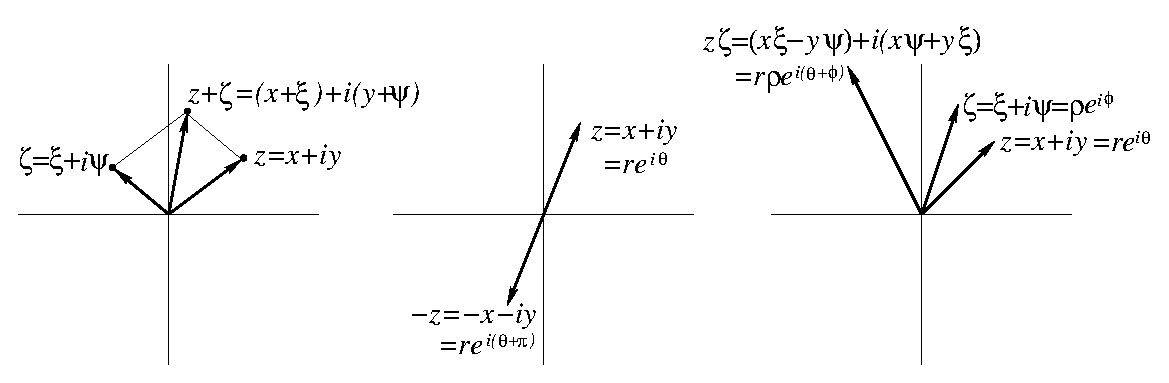
\includegraphics[width=\textwidth]{fcv/number/add_neg_mult}
  \end{center}
  \caption{Addition, negation and multiplication.}
  \label{add_neg_mult}
\end{figure}







\paragraph{Multiplicative inverse.}
Assume that $z$ is nonzero.  The multiplicative inverse of 
$z = r \e^{\imath \theta}$ is $\frac{1}{z} = \frac{1}{r} \e^{-\imath \theta}$.
The length of $\frac{1}{z}$ is the multiplicative inverse of the length
of $z$.  The angle of $\frac{1}{z}$ is the negative of the angle of $z$.
(See Figure~\ref{inv_div_conj}.)







\paragraph{Division.}
Assume that $\zeta$ is nonzero.
The quotient of $z = r \e^{\imath \theta}$ and $\zeta = \rho \e^{\imath \phi}$ is
$\frac{z}{\zeta} = \frac{r}{\rho} \e^{ \imath (\theta - \phi)}$.  The length of 
the vector $\frac{z}{\zeta}$ is the quotient of the lengths of 
$z$ and $\zeta$.  The angle of $\frac{z}{\zeta}$ is the difference of the 
angles of $z$ and $\zeta$.
(See Figure~\ref{inv_div_conj}.)





\paragraph{Complex conjugate.}
The complex conjugate of $z = x + \imath y = r \e^{\imath \theta}$ is 
$\overline{z} = x - \imath y = r \e^{-\imath \theta}$.  $\overline{z}$ is the mirror image of
$z$, reflected across the $x$ axis.  In other words, $\overline{z}$ has the
same magnitude as $z$ and the angle of $\overline{z}$ is the negative of 
the angle of $z$.
(See Figure~\ref{inv_div_conj}.)

\begin{figure}[h!]
  \begin{center}
      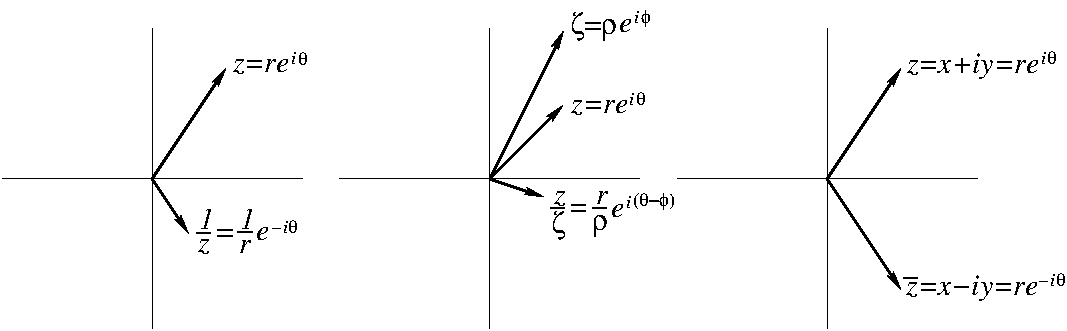
\includegraphics[width=\textwidth]{fcv/number/inv_div_conj}
  \end{center}
  \caption{Multiplicative inverse, division and complex conjugate.}
  \label{inv_div_conj}
\end{figure}

















%%=============================================================================
\section{Integer Exponents}





Consider the product $(a + b)^n$, $n \in \mathbb{Z}$.  
If we know $\arctan(a,b)$ then 
it will be most convenient to expand the product working in polar form.  
If not, we can write $n$ in base 2 to efficiently do the multiplications.




\begin{Example}
  Suppose that we want to write $\left( \sqrt{3} + \imath \right)^{20}$ 
  in Cartesian form.%
  \footnote{No, I have no idea why we would want to do that.  Just humor
    me.  If you pretend that you're interested, I'll do the same.  Believe
    me, expressing your real feelings here isn't going to do anyone any good.}
  We can do the multiplication directly.  Note that $20$ is $10100$ in base 2.
  That is, $20 = 2^4 + 2^2$.  We first calculate the powers of the form
  $\left( \sqrt{3} + \imath \right)^{2^n}$ by successive squaring.
  \begin{align*}
    \left( \sqrt{3} + \imath \right)^2 &= 2 + \imath 2 \sqrt{3} \\
    \left( \sqrt{3} + \imath \right)^4 &= -8 + \imath 8 \sqrt{3} \\
    \left( \sqrt{3} + \imath \right)^8 &= -128 - \imath 128 \sqrt{3} \\
    \left( \sqrt{3} + \imath \right)^{16} &= -32768 + \imath 32768 \sqrt{3} 
  \end{align*}
  Next we multiply $\left( \sqrt{3} + \imath \right)^4$ and 
  $\left( \sqrt{3} + \imath \right)^{16}$ to obtain the answer.
  \[
  \left( \sqrt{3} + \imath \right)^{20} 
  = \left( -32768 + \imath 32768 \sqrt{3} \right) 
  \left( - 8 + \imath 8 \sqrt{3} \right)
  = - 524288 - \imath 524288 \sqrt{3}
  \]

  Since we know that $\arctan\left( \sqrt{3},1 \right) = \pi/6$,
  it is easiest to do this problem by first changing to modulus-argument form.
  \begin{align*}
    \left( \sqrt{3} + \imath \right)^{20} 
    &= \left( \sqrt{ \left( \sqrt{3} \right)^2 + 1^2} 
      \e^{\imath \arctan(\sqrt{3},1)} \right)^{20} 
    \\
    &= \left( 2 \e^{\imath \pi / 6} \right)^{20} 
    \\
    &= 2^{20} \e^{\imath 4 \pi / 3} 
    \\
    &= 1048576 \left( - \frac{1}{2} - \imath \frac{\sqrt{3}}{2} \right) 
    \\
    &= - 524288 - \imath 524288 \sqrt{3}
  \end{align*}
\end{Example}








\begin{Example}
  Consider $(5 + \imath 7)^{11}$.  We will do the exponentiation in polar form and
  write the result in Cartesian form.
  \begin{align*}
    (5 + \imath 7)^{11}
    &= \left( \sqrt{74} \e^{\imath \arctan(5,7)} \right)^{11} \\
    &= 74^5 \sqrt{74} ( \cos( 11 \arctan(5,7)) 
    + \imath \sin( 11 \arctan(5,7)))\\
    &= 2219006624 \sqrt{74} \cos( 11 \arctan(5,7))
    + \imath 2219006624 \sqrt{74} \sin( 11 \arctan(5,7))
  \end{align*}
  The result is correct, but not very satisfying.
  This expression could be simplified.
  You could evaluate the trigonometric functions with some fairly messy
  trigonometric identities.  This would take much more work than directly 
  multiplying $(5 + \imath 7)^{11}$.
\end{Example}












%%=============================================================================
\section{Rational Exponents}





In this section we consider complex numbers with rational exponents,
$z^{p/q}$, where $p/q$ is a rational number.  First we consider unity 
raised to the $1/n$ power.   We define $1^{1/n}$ as the set of numbers
$\{z\}$ such that $z^n = 1$.
\[
1^{1/n} = \left\{ z \mid z^n = 1 \right\}
\]
We can find these values by writing $z$ in modulus-argument form.
\begin{gather*}
  z^n = 1 
  \\
  r^n \e^{\imath n \theta} = 1 
  \\
  r^n = 1 \qquad n \theta = 0 \mod 2 \pi 
  \\
  r = 1 \qquad \theta = 2 \pi k\ \mathrm{for}\ k \in \mathbb{Z}
  \\
  1^{1/n} = \left\{ \e^{\imath 2 \pi k/n} \mid k \in \mathbb{Z} \right\} 
\end{gather*}
There are only $n$ distinct values as a result of the $2 \pi$ periodicity 
of $\e^{\imath \theta}$. $\e^{\imath 2 \pi} = \e^{\imath 0}$.
\[
1^{1/n} = \left\{ \e^{\imath 2 \pi k / n} \mid k = 0, \ldots, n-1 \right\}
\]
These values are equally spaced points on the unit circle in the 
complex plane.



\begin{Example}
  $1^{1/6}$ has the 6 values,
  \[
  \left\{ \e^{\imath 0}, \e^{\imath \pi/3}, \e^{\imath 2 \pi/3}, \e^{\imath \pi}, \e^{\imath 4 \pi/3},
    \e^{\imath 5 \pi/3} \right\}.
  \]
  In Cartesian form this is
  \[
  \left\{ 1, \frac{1 + \imath \sqrt{3}}{2}, \frac{-1 + \imath \sqrt{3}}{2},
    -1, \frac{-1 - \imath \sqrt{3}}{2}, \frac{1 - \imath \sqrt{3}}{2} \right\}.
  \]
  The sixth roots of unity are plotted in Figure~\ref{sixth_roots}.
  \begin{figure}[h!]
    \begin{center}
        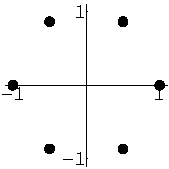
\includegraphics[width=0.2\textwidth]{fcv/number/sixth_roots}
    \end{center}
    \caption{The sixth roots of unity.}
    \label{sixth_roots}
  \end{figure}
\end{Example}




The $n^{\mathrm{th}}$ roots of the complex number $c = \alpha \e^{\imath \beta}$
are the set of numbers $z = r \e^{\imath \theta}$ such that
\begin{gather*}
  z^n = c = \alpha \e^{\imath \beta} 
  \\
  r^n \e^{\imath n \theta} = \alpha \e^{\imath \beta} 
  \\
  r = \sqrt[n]{\alpha} \qquad n \theta = \beta \mod 2 \pi 
  \\
  r = \sqrt[n]{\alpha} \qquad \theta = (\beta + 2 \pi k) / n\ \mathrm{for}\ 
  k = 0, \ldots, n - 1.
\end{gather*}
Thus 
\[
c^{1/n} = \left\{ \sqrt[n]{\alpha} \e^{\imath (\beta + 2 \pi k) / n } \mid k = 0, \ldots, n - 1 \right\}
= \left\{ \sqrt[n]{|c|} \e^{\imath (\Arg(c) + 2 \pi k) / n } \mid k = 0, \ldots, n - 1 \right\}
\]


\paragraph{Principal roots.}
The \textit{principal $n^{\mathrm{th}}$ root} is denoted
\index{principal root}
\[
\sqrt[n]{z} \equiv \sqrt[n]{z} \e^{\imath \Arg(z) / n}.
\]
Thus the principal root has the property
\[
- \pi / n < \Arg \left( \sqrt[n]{z} \right) \leq \pi / n.
\]
This is consistent with the notation from functions of a real variable:
$\sqrt[n]{x}$ denotes the positive $n^{\mathrm{th}}$ root of a positive 
real number.  We adopt the convention that $z^{1/n}$ denotes the 
$n^{\mathrm{th}}$ roots of $z$, which is a set of $n$ numbers and 
$\sqrt[n]{z}$ is the principal $n^{\mathrm{th}}$ root of $z$, which is a 
single number.  
The $n^{\mathrm{th}}$ roots of $z$ are the principal $n^{\mathrm{th}}$
root of $z$ times the $n^{\mathrm{th}}$ roots of unity.
\begin{gather*}
  z^{1/n} = \left\{ \sqrt[n]{r} \e^{\imath (\Arg(z) + 2 \pi k) / n } \mid k = 0, \ldots, n-1 \right\} 
  \\
  z^{1/n} = \left\{ \sqrt[n]{z} \e^{\imath 2 \pi k / n } \mid k = 0, \ldots, n-1 \right\} 
  \\
  z^{1/n} = \sqrt[n]{z} 1^{1/n}
\end{gather*}




\paragraph{Rational exponents.}
We interpret $z^{p/q}$ to mean $z^{(p/q)}$.  That is, we first simplify
the exponent, i.e. reduce the fraction,  before carrying out the 
exponentiation.  Therefore $z^{2/4} = z^{1/2}$ and $z^{10/5} = z^2$.
If $p/q$ is a reduced fraction, ($p$ and $q$ are relatively prime, in other
words, they have no common factors), then 
\[
z^{p/q} \equiv \left( z^p \right)^{1/q}.
\]
Thus $z^{p/q}$ is a set of $q$ values.  Note that for an un-reduced fraction
$r/s$, 
\[
\left( z^r \right)^{1/s} \neq \left( z^{1/s} \right)^r.
\]
The former expression is a set of $s$ values while the latter is a set of
no more that $s$ values.  For instance, $\left( 1^2 \right)^{1/2} = 1^{1/2} = \pm 1$
and $\left( 1^{1/2} \right)^2 = (\pm 1)^2 = 1$.






\begin{Example}
  Consider $2^{1/5}$, $(1 + \imath)^{1/3}$ and $(2 + \imath)^{5/6}$.
  \[
  2^{1/5} = \sqrt[5]{2} \e^{\imath 2 \pi k / 5}, \quad \mathrm{for}\ k = 0,1,2,3,4
  \]
  \begin{align*}
    (1 + \imath)^{1/3}
    &= \left( \sqrt{2} \e^{\imath \pi/4} \right)^{1/3} 
    \\
    &= \sqrt[6]{2} \e^{\imath \pi / 12} \e^{\imath 2 \pi k / 3}, \quad \mathrm{for}\ k = 0, 1, 2
  \end{align*}
  \begin{align*}
    (2 + \imath)^{5/6}
    &= \left( \sqrt{5} \e^{\imath \Arctan(2,1) } \right)^{5/6} 
    \\
    &= \left( \sqrt{5^5} \e^{\imath 5 \Arctan(2,1) } \right)^{1/6} 
    \\
    &= \sqrt[12]{5^5} \e^{\imath \frac{5}{6} \Arctan(2,1)}
    \e^{\imath \pi k / 3}, \quad \mathrm{for}\ k = 0,1,2,3,4,5
  \end{align*}
\end{Example}





\begin{Example}
  We find the roots of $z^5 + 4$.
  \begin{align*}
    (- 4)^{1/5}
    &= \left( 4 \e^{\imath \pi} \right)^{1/5} 
    \\
    &= \sqrt[5]{4} \e^{\imath \pi (1 + 2 k) / 5}, \quad \mathrm{for}\ k = 0,1,2,3,4
  \end{align*}
\end{Example}













\raggedbottom
%%=============================================================================
\exercises{
\pagebreak
\flushbottom
\section{Exercises}




%%-----------------------------------------------------------------------------
\begin{large}
  \noindent
  \textbf{Complex Numbers}
\end{large}





\begin{Exercise}
  \label{exercise 1i27}
  If $z = x + \imath y$, write the following in the form $a + \imath b$:
  \begin{enumerate}
  \item
    $\displaystyle
    (1 + \imath 2)^7
    $
  \item
    $\displaystyle
    \frac{1}{ \left( \overline{z} \overline{z} \right) }
    $
  \item
    $\displaystyle
    \frac{ \imath z + \overline{z} }{ (3 + \imath)^9 }
    $
  \end{enumerate}

  \hintsolution{1i27}
\end{Exercise}







%% \frac{1 + \imath 2}{3 - \imath 4} + \frac{2-\imath}{\imath 5} = - \frac{2}{5}
\begin{Exercise}
  \label{exercise (1 - i)4 = -4}
  Verify that:
  \begin{enumerate}
  \item
    $\displaystyle \frac{1 + \imath 2}{3 - \imath 4} + \frac{2 - \imath}{\imath 5} 
    = - \frac{2}{5}$
  \item
    $\displaystyle (1 - \imath)^4 = - 4$
  \end{enumerate}

  \hintsolution{(1 - i)4 = -4}
\end{Exercise}






%% \left( 1 + \imath \sqrt{3} \right)^{-10}
\begin{Exercise}
  \label{exercise (11 + i4)2}
  Write the following complex numbers in the form $a + \imath b$.
  \begin{enumerate}
  \item
    $\displaystyle \left( 1 + \imath \sqrt{3} \right)^{-10}$
  \item
    $\displaystyle (11 + \imath 4)^2$
  \end{enumerate}

  \hintsolution{(11 + i4)2}
\end{Exercise}





%% \left( \frac{2 + \imath}{\imath 6 - (1 - \imath 2)} \right)^2
\begin{Exercise}
  \label{exercise (1 - i)7}
  Write the following complex numbers in the form $a + \imath b$
  \begin{enumerate}
  \item
    $\displaystyle
    \left( \frac{2 + \imath}{\imath 6 - (1 - \imath 2)} \right)^2
    $
  \item
    $\displaystyle
    (1 - \imath)^7
    $
  \end{enumerate}

  \hintsolution{(1 - i)7}
\end{Exercise}








%% \overline{ \left( \frac{ \overline{z} }{ z } \right) }$
\begin{Exercise}
  \label{exercise ov ov z z}
  If $z = x + \imath y$, write the following in the form $u(x,y) + \imath v(x,y)$.
  \begin{enumerate}
  \item
    $\displaystyle 
    \overline{ \left( \frac{ \overline{z} }{ z } \right) }
    $
  \item
    $\displaystyle 
    \frac{ z + \imath 2 }{ 2 - \imath \overline{z} }
    $
  \end{enumerate}

  \hintsolution{ov ov z z}
\end{Exercise}







%% Quaternions are sometimes used as a generalization of complex numbers.
\begin{Exercise}
  \label{exercise quaternion}
  Quaternions are sometimes used as a generalization of complex numbers.
  A quaternion $u$ may be defined as
  \[
  u = u_0 + \imath u_1 + \jmath u_2 + k u_3
  \]
  where $u_0$, $u_1$, $u_2$ and $u_3$ are real numbers and $\imath$, $\jmath$ and $k$
  are objects which satisfy
  \[
  \imath^2 = \jmath^2 = k^2 = -1, \quad
  \imath \jmath = k, \quad
  \jmath \imath = - k
  \]
  and the usual associative and distributive laws.  Show that for any
  quaternions $u$, $w$ there exists a quaternion $v$ such that
  \[
  u v = w
  \]
  except for the case $u_0 = u_1 = u_2 = u_3$.

  \hintsolution{quaternion}
\end{Exercise}






%% $\alpha = t\beta$ $\Im(\alpha\overline{\beta}) = 0$
\begin{Exercise}
  \label{exercise alpha = t beta}
  Let $\alpha \neq 0$, $\beta \neq 0$ be two complex numbers.
  Show that $\alpha = t \beta$ for some real number $t$ (i.e. the vectors
  defined by $\alpha$ and $\beta$ are parallel) if and only if
  $\Im\left( \alpha \overline{\beta} \right) = 0$.

  \hintsolution{alpha = t beta}
\end{Exercise}







%%-----------------------------------------------------------------------------
\begin{large}
  \noindent
  \textbf{The Complex Plane}
\end{large}




\begin{Exercise}
  \label{exercise 1i13}
  Find and depict all values of
  \begin{enumerate}
  \item
    $\displaystyle
    (1 + \imath)^{1/3}
    $
  \item
    $\displaystyle
    \imath^{1/4}
    $
  \end{enumerate}
  Identify the principal root.

  \hintsolution{1i13}
\end{Exercise}






\begin{Exercise}
  \label{exercise Rez+2Imz1}
  Sketch the regions of the complex plane:
  \begin{enumerate}
  \item
    $\displaystyle
    | \Re(z) | + 2 | \Im(z) | \leq 1
    $
  \item
    $\displaystyle
    1 \leq |z - \imath| \leq 2
    $
  \item
    $\displaystyle
    |z - \imath| \leq |z + \imath|
    $
  \end{enumerate}

  \hintsolution{Rez+2Imz1}
\end{Exercise}








%% argument identities
\begin{Exercise}
  \label{exercise argument identities}
  Prove the following identities.
  \begin{enumerate}
  \item
    $\arg(z \zeta) = \arg(z) + \arg(\zeta)$
  \item
    $\Arg(z \zeta) \neq \Arg(z) + \Arg(\zeta)$
  \item
    $\arg \left( z^2 \right) = \arg(z) + \arg(z) \neq 2 \arg(z)$
  \end{enumerate}

  \hintsolution{argument identities}
\end{Exercise}




%% triangle inequalities
\begin{Exercise}
  \label{exercise triangle inequalities}
  Show, both by geometric and algebraic arguments, that
  for complex numbers $z$ and $\zeta$ the inequalities
  \[
  ||z|-|\zeta||\leq |z + \zeta|\leq |z| + |\zeta|
  \]
  hold.

  \hintsolution{triangle inequalities}
\end{Exercise}





%% $(-1)^{-3/4}$ $8^{1/6}$
\begin{Exercise}
  \label{exercise -1 -3/4 8 1/6}
  Find all the values of
  \begin{enumerate}
  \item
    $(- 1)^{-3/4}$
  \item
    $8^{1/6}$
  \end{enumerate}
  and show them graphically.

  \hintsolution{-1 -3/4 8 1/6}
\end{Exercise}







%% (-1)^{-1/4}
\begin{Exercise}
  \label{exercise 16 1/8}
  Find all values of
  \begin{enumerate}
  \item
    $ \displaystyle
    (- 1)^{-1/4}
    $
  \item
    $ \displaystyle
    16^{1/8}
    $
  \end{enumerate}
  and show them graphically.

  \hintsolution{16 1/8}
\end{Exercise}



%% $1 < |z - 2 \imath| < 2$ $| \Re(z) | + 5 | \Im(z) | = 1$
\begin{Exercise}
  \label{exercise 1 z-i2 2}
  Sketch the regions or curves described by
  \begin{enumerate}
  \item
    $\displaystyle
    1 < |z - \imath 2| < 2
    $
  \item
    $\displaystyle
    | \Re(z) | + 5 | \Im(z) | = 1
    $
  \item
    $\displaystyle
    |z - \imath|=|z + \imath|
    $
  \end{enumerate}

  \hintsolution{1 z-i2 2}
\end{Exercise}




%% |z - 1 + \imath|\leq 1
\begin{Exercise}
  \label{exercise z-1+i 1}
  Sketch the regions or curves described by
  \begin{enumerate}
  \item
    $\displaystyle
    |z - 1 + \imath|\leq 1
    $
  \item
    $\displaystyle
    \Re(z)- \Im(z) = 5
    $
  \item
    $\displaystyle
    |z - \imath| + |z + \imath| = 1
    $
  \end{enumerate}

  \hintsolution{z-1+i 1}
\end{Exercise}





%% |\e^{\imath \theta}-1| =2
\begin{Exercise}
  \label{exercise e i theta - 1 = 2}
  Solve the equation
  \[
  |\e^{\imath \theta}-1| = 2
  \]
  for $\theta$ ($0 \leq \theta \leq \pi$) and verify the solution geometrically.

  \hintsolution{e i theta - 1 = 2}
\end{Exercise}






%%-----------------------------------------------------------------------------
\begin{large}
  \noindent
  \textbf{Polar Form}
\end{large}



%% Euler's formula
\begin{Exercise}
  \label{exercise eulers formula}
  Show that Euler's formula, $\e^{\imath \theta} = \cos \theta + \imath \sin \theta$, is
  formally consistent with the standard Taylor series expansions for
  the real functions $\e^x$, $\cos x$ and $\sin x$.  Consider the
  Taylor series of $\e^x$ about $x = 0$ to be the definition of the
  exponential function for complex argument.

  \hintsolution{eulers formula}
\end{Exercise}





%% \cos(3\theta) = \cos^3(\theta) -3\cos(\theta)\sin^2(\theta).
\begin{Exercise}
  \label{exercise cos 3t = cos3 t - 3 cos t sin2 t}
  Use de Moivre's formula to derive the 
  trigonometric identity
  \[
  \cos(3 \theta) = \cos^3(\theta) - 3 \cos(\theta) \sin^2(\theta).
  \]

  \hintsolution{cos 3t = cos3 t - 3 cos t sin2 t}
\end{Exercise}







%% 1 + z + z^2 + \cdots + z^n = \frac{1 - z^{n+1}}{1-z}, \qquad (z \neq 1),
\begin{Exercise}
  \label{exercise geometric trig identity}
  Establish the formula
  \[
  1 + z + z^2 + \cdots + z^n = \frac{1 - z^{n+1}}{1-z}, \qquad (z \neq 1),
  \]
  for the sum of a finite geometric series;  then derive the formulas
  \begin{enumerate}
  \item
    $\displaystyle 
    1 + \cos(\theta) + \cos(2 \theta) + \cdots + \cos(n \theta) 
    = \frac{1}{2} + \frac{\sin( ( n + 1/2 ) )} { 2 \sin (\theta / 2) }
    $
  \item
    $\displaystyle 
    \sin(\theta) + \sin(2 \theta) + \cdots + \sin(n \theta) 
    = \frac{1}{2} \cot \frac{\theta}{2}
    - \frac{\cos( ( n + 1/2 ) )} { 2 \sin (\theta / 2) }
    $
  \end{enumerate}
  where $0 < \theta < 2 \pi$.

  \hintsolution{geometric trig identity}
\end{Exercise}






%%-----------------------------------------------------------------------------
\begin{large}
  \noindent
  \textbf{Arithmetic and Vectors}
\end{large}


%% modulus identities with polar form
\begin{Exercise}
  \label{exercise modulus identities polar}
  Prove $|z \zeta| = |z| |\zeta|$ and $\left| \frac{z}{\zeta} \right|
  = \frac{|z|}{|\zeta|}$ using polar form.

  \hintsolution{modulus identities polar}
\end{Exercise}






%% parallelogram identity
\begin{Exercise}
  \label{exercise parallelogram identity}
  Prove that 
  \[
  \left| z + \zeta \right|^2 + \left| z - \zeta \right|^2
  = 2 \left( \left| z \right|^2 + \left| \zeta \right|^2 \right).
  \]
  Interpret this geometrically.

  \hintsolution{parallelogram identity}
\end{Exercise}







%%-----------------------------------------------------------------------------
\begin{large}
  \noindent
  \textbf{Integer Exponents}
\end{large}



%% (1 + \imath)^{10}
\begin{Exercise}
  \label{exercise (1+i)10}
  Write $(1 + \imath)^{10}$ in Cartesian form with the following two methods:
  \begin{enumerate}
  \item
    Just do the multiplication.  If it takes you more than four 
    multiplications, you suck.
  \item
    Do the multiplication in polar form.
  \end{enumerate}

  \hintsolution{(1+i)10}
\end{Exercise}




%%-----------------------------------------------------------------------------
\begin{large}
  \noindent
  \textbf{Rational Exponents}
\end{large}




%% Quadratic formula
\begin{Exercise}
  \label{exercise z2 + 2az + b = 0}
  Show that each of the numbers $z = - a + \left( a^2 - b \right)^{1/2}$ 
  satisfies the equation $z^2 + 2 a z + b = 0$.

  \hintsolution{z2 + 2az + b = 0}
\end{Exercise}




















\raggedbottom
}
%%=============================================================================
\hints{
\pagebreak
\flushbottom
\section{Hints}






%%-----------------------------------------------------------------------------
\begin{large}
  \noindent
  \textbf{Complex Numbers}
\end{large}




\begin{Hint}
  \label{hint 1i27}
  %% CONTINUE
\end{Hint}





%% \frac{1 + \imath 2}{3 - \imath 4} + \frac{2 - \imath}{\imath 5} = - \frac{2}{5}
\begin{Hint}
  \label{hint (1 - i)4 = -4}
  %% CONTINUE
\end{Hint}




%% \left( 1 + \imath \sqrt{3} \right)^{-10}
\begin{Hint}
  \label{hint (11 + i4)2}
  %% CONTINUE
\end{Hint}




%% \left( \frac{2 + \imath}{\imath 6 - (1 - \imath 2)} \right)^2
\begin{Hint}
  \label{hint (1 - i)7}
  %% CONTINUE
\end{Hint}





%% \overline{ \left( \frac{ \overline{z} }{ z } \right) }$
\begin{Hint}
  \label{hint ov ov z z}
  %% CONTINUE
\end{Hint}






%% Quaternions are sometimes used as a generalization of complex numbers.
\begin{Hint}
  \label{hint quaternion}
  %% CONTINUE
\end{Hint}





%% $\alpha = t\beta$ $\Im(\alpha\overline{\beta}) = 0$
\begin{Hint}
  \label{hint alpha = t beta}
  %% CONTINUE
\end{Hint}




%%-----------------------------------------------------------------------------
\begin{large}
  \noindent
  \textbf{The Complex Plane}
\end{large}


\begin{Hint}
  \label{hint 1i13}
  %% CONTINUE
\end{Hint}



\begin{Hint}
  \label{hint Rez+2Imz1}
  %% CONTINUE
\end{Hint}





%% argument identities
\begin{Hint}
  \label{hint argument identities}
  Write the multivaluedness explicitly.
\end{Hint}




%% triangle inequalities
\begin{Hint}
  \label{hint triangle inequalities}
  Consider a triangle with vertices at $0$, $z$ and $z + \zeta$.
\end{Hint}





%% $(-1)^{-3/4}$ $8^{1/6}$
\begin{Hint}
  \label{hint -1 -3/4 8 1/6}
  %% CONTINUE
\end{Hint}


%% (-1)^{-1/4}
\begin{Hint}
  \label{hint 16 1/8}
  %% CONTINUE
\end{Hint}




%% $1 < |z - 2 \imath| < 2$ $| \Re(z) | + 5 | \Im(z) | = 1$
\begin{Hint}
  \label{hint 1 z-i2 2}
  %% CONTINUE
\end{Hint}


%% |z - 1 + \imath|\leq 1
\begin{Hint}
  \label{hint z-1+i 1}
  %% CONTINUE
\end{Hint}




%% |\e^{\imath \theta}-1| =2
\begin{Hint}
  \label{hint e i theta - 1 = 2}
  %% CONTINUE
\end{Hint}





%%-----------------------------------------------------------------------------
\begin{large}
  \noindent
  \textbf{Polar Form}
\end{large}




%% Euler's formula
\begin{Hint}
  \label{hint eulers formula}
  Find the Taylor series of $\e^{\imath \theta}$, $\cos \theta$ and $\sin \theta$.
  Note that $\imath^{2 n} = (- 1)^n$.
\end{Hint}





%% \cos(3\theta) = \cos^3(\theta) -3\cos(\theta)\sin^2(\theta).
\begin{Hint}
  \label{hint cos 3t = cos3 t - 3 cos t sin2 t}
  %% CONTINUE
\end{Hint}






%% 1 + z + z^2 + \cdots + z^n = \frac{1 - z^{n+1}}{1-z}, \qquad (z \neq 1),
\begin{Hint}
  \label{hint geometric trig identity}
  %% CONTINUE
\end{Hint}








%%-----------------------------------------------------------------------------
\begin{large}
  \noindent
  \textbf{Arithmetic and Vectors}
\end{large}


%% modulus identities with polar form
\begin{Hint}
  \label{hint modulus identities polar}
  $|\e^{\imath \theta} | = 1$.
\end{Hint}




%% parallelogram identity
\begin{Hint}
  \label{hint parallelogram identity}
  Consider the parallelogram defined by $z$ and $\zeta$.
\end{Hint}






%%-----------------------------------------------------------------------------
\begin{large}
  \noindent
  \textbf{Integer Exponents}
\end{large}


%% (1 + \imath)^{10}
\begin{Hint}
  \label{hint (1+i)10}
  For the first part,
  \[
  (1 + \imath)^{10} = \left( \left( (1 + \imath)^2 \right)^2 \right)^2 (1 + \imath)^2.
  \]
\end{Hint}



%%-----------------------------------------------------------------------------
\begin{large}
  \noindent
  \textbf{Rational Exponents}
\end{large}




%% Quadratic formula
\begin{Hint}
  \label{hint z2 + 2az + b = 0}
  Substitite the numbers into the equation.
\end{Hint}


























\raggedbottom
}
%%=============================================================================
\solutions{
\pagebreak
\flushbottom
\section{Solutions}





%%-----------------------------------------------------------------------------
\begin{large}
  \noindent
  \textbf{Complex Numbers}
\end{large}






\begin{Solution}
  \label{solution 1i27}
  \begin{enumerate}
  \item
    We can do the exponentiation by directly multiplying.
    \begin{align*}
      (1 + \imath 2)^7
      &= (1 + \imath 2)  (1 + \imath 2)^2  (1 + \imath 2)^4
      \\
      &= (1 + \imath 2)  (-3 + \imath 4)  (-3 + \imath 4)^2
      \\
      &= (11 - \imath 2)  (-7 - \imath 24)
      \\
      &= 29 + \imath 278
    \end{align*}
    We can also do the problem using De Moivre'{}s Theorem.
    \begin{align*}
      (1 + \imath 2)^7
      &= \left( \sqrt{5} \e^{\imath \arctan(1,2)} \right)^7
      \\
      &= 125 \sqrt{5} \e^{\imath 7 \arctan(1,2)}
      \\
      &= 125 \sqrt{5} \cos(7 \arctan(1,2)) 
      + \imath 125 \sqrt{5} \sin(7 \arctan(1,2))
    \end{align*}
    
  \item
    \begin{align*}
      \frac{1}{ \left( \overline{z} \overline{z} \right) }
      &= \frac{1}{ (x - \imath y)^2 }
      \\
      &= \frac{1}{ (x - \imath y)^2 }  \frac{ (x + \imath y)^2 }{ (x + \imath y)^2 }
      \\
      &= \frac{ (x + \imath y)^2 }{ (x^2 + y^2)^2 }
      \\
      &= \frac{ x^2 - y^2 }{ (x^2 + y^2)^2 }
      + \imath \frac{ 2 x y }{ (x^2 + y^2)^2 }
    \end{align*}
  \item
    We can evaluate the expression using De Moivre'{}s Theorem.
    \begin{align*}
      \frac{ \imath z + \overline{z} }{ (3 + \imath)^9 }
      &= (-y + \imath x + x - \imath y) (3 + \imath)^{-9}
      \\
      &= (1 + \imath) (x - y) \left( \sqrt{10} \e^{\imath \arctan(3,1)} \right)^{-9}
      \\
      &= (1 + \imath) (x - y) \frac{1}{10000 \sqrt{10}} \e^{-\imath 9 \arctan(3,1)}
      \\
      &= \frac{ (1 + \imath) (x - y) }{ 10000 \sqrt{10} } 
      \left( \cos(9 \arctan(3,1)) - \imath \sin(9 \arctan(3,1)) \right)
      \\
      &= \frac{(x - y)}{10000 \sqrt{10}} \left( \cos(9 \arctan(3,1))
        + \sin(9 \arctan(3,1)) \right)
      \\
      &\qquad+ \imath \frac{(x - y)}{10000 \sqrt{10}} \left( \cos(9 \arctan(3,1))
        - \sin(9 \arctan(3,1)) \right)
    \end{align*}
    We can also do this problem by directly multiplying but it's a 
    little grungy.
    \begin{align*}
      \frac{ \imath z + \overline{z} }{ (3 + \imath)^9 }
      &= \frac{ (-y + \imath x + x - \imath y) (3 - \imath)^9 }{ 10^9 }
      \\
      &= \frac{ (1 + \imath) (x - y) (3 - \imath) \left( \left( (3 - \imath)^2 \right)^2 
        \right)^2}{ 10^9 }
      \\
      &= \frac{ (1 + \imath) (x - y) (3 - \imath) \left( \left( 8 - \imath 6 \right)^2 
        \right)^2}{ 10^9 }
      \\
      &= \frac{ (1 + \imath) (x - y) (3 - \imath) ( 28 - \imath 96 )^2}{ 10^9 }
      \\
      &= \frac{ (1 + \imath) (x - y) (3 - \imath) ( -8432 - \imath 5376)}{ 10^9 }
      \\
      &= \frac{ (x - y) (-22976 - \imath 38368) }{ 10^9 }
      \\
      &= \frac{ 359 (y - x) }{ 15625000 } + \imath \frac{ 1199 (y-x) }{ 31250000 }
    \end{align*}
  \end{enumerate}
\end{Solution}







%% \frac{1 + \imath 2}{3 - \imath 4} + \frac{2 - \imath}{\imath 5} = - \frac{2}{5}
\begin{Solution}
  \label{solution (1 - i)4 = -4}
  \begin{enumerate}
  \item
    \begin{align*}
      \frac{1 + \imath 2}{3 - \imath 4} + \frac{2 - \imath}{\imath 5} 
      &= \frac{1 + \imath 2}{3 - \imath 4}  \frac{3 + \imath 4}{3 + \imath 4} 
      + \frac{2 - \imath}{\imath 5}  \frac{- \imath}{- \imath} 
      \\
      &= \frac{-5 + \imath 10}{25} + \frac{-1 - \imath 2}{5} 
      \\
      &= - \frac{2}{5}
    \end{align*}
  \item
    \[
    (1 - \imath)^4 = (- \imath 2)^2 = - 4
    \]
  \end{enumerate}
\end{Solution}







%% \left( 1 + \imath \sqrt{3} \right)^{-10}
\begin{Solution}
  \label{solution (11 + i4)2}
  \begin{enumerate}
  \item
    First we do the multiplication in Cartesian form.
    \begin{align*}
      \left( 1 + \imath \sqrt{3} \right)^{-10}
      &= \left( \left( 1 + \imath \sqrt{3} \right)^2 
        \left( 1 + \imath \sqrt{3} \right)^8 \right)^{-1} 
      \\
      &= \left( \left( - 2 + \imath 2 \sqrt{3} \right) 
        \left( - 2 + \imath 2 \sqrt{3} \right)^4 \right)^{-1} 
      \\
      &= \left( \left( - 2 + \imath 2 \sqrt{3} \right) 
        \left( - 8 - \imath 8 \sqrt{3} \right)^2 \right)^{-1} 
      \\
      &= \left( \left( - 2 + \imath 2 \sqrt{3} \right) 
        \left( - 128 + \imath 128 \sqrt{3} \right) \right)^{-1} 
      \\
      &= \left( - 512 - \imath 512 \sqrt{3} \right)^{-1} 
      \\
      &= \frac{1}{512}  \frac{- 1}{1 + \imath \sqrt{3}} 
      \\
      &= \frac{1}{512}  \frac{- 1}{1 + \imath \sqrt{3}} 
       \frac{1 - \imath \sqrt{3}}{1 - \imath \sqrt{3}} 
      \\
      &= - \frac{1}{2048} + \imath \frac{\sqrt{3}}{2048}
    \end{align*}

    Now we do the multiplication in modulus-argument, (polar), form.
    \begin{align*}
      \left( 1 + \imath \sqrt{3} \right)^{-10}
      &= \left( 2 \e^{\imath \pi / 3} \right)^{-10} 
      \\
      &= 2^{-10} \e^{- \imath 10 \pi / 3} 
      \\
      &= \frac{1}{1024} \left( \cos \left( - \frac{10 \pi}{3} \right)
        + \imath \sin \left( - \frac{10 \pi}{3} \right) \right) 
      \\
      &= \frac{1}{1024} \left( \cos \left( \frac{4 \pi}{3} \right)
        - \imath \sin \left( \frac{4 \pi}{3} \right) \right) 
      \\
      &= \frac{1}{1024} \left( - \frac{1}{2} + \imath \frac{\sqrt{3}}{2} \right)
      \\
      &= - \frac{1}{2048} + \imath \frac{\sqrt{3}}{2048}
    \end{align*}
  \item
    \[
    (11 + \imath 4)^2 = 105 + \imath 88
    \]
  \end{enumerate}
\end{Solution}




%% \left( \frac{2 + \imath}{\imath 6 - (1 - \imath 2)} \right)^2
\begin{Solution}
  \label{solution (1 - i)7}
  \begin{enumerate}
  \item
    \begin{align*}
      \left( \frac{2 + \imath}{\imath 6 -(1 - \imath 2)} \right)^2
      &= \left( \frac{2 + \imath}{- 1 + \imath 8} \right)^2 
      \\
      &= \frac{3 + \imath 4}{- 63 - \imath 16} 
      \\
      &= \frac{3 + \imath 4}{- 63 - \imath 16}  \frac{- 63 + \imath 16}{- 63 + \imath 16} 
      \\
      &= - \frac{253}{4225} - \imath \frac{204}{4225}
    \end{align*}
  \item
    \begin{align*}
      (1 - \imath)^7
      &= \left( (1 - \imath)^{2} \right)^2  (1 - \imath)^2  (1 - \imath) 
      \\
      &= (- \imath 2)^2  (- \imath 2)  (1 - \imath) 
      \\
      &= (- 4)  (- 2 - \imath 2) 
      \\
      &= 8 + \imath 8
    \end{align*}
  \end{enumerate}
\end{Solution}














%% \overline{ \left( \frac{ \overline{z} }{ z } \right) }$
\begin{Solution}
  \label{solution ov ov z z}
  \begin{enumerate}
    %%
  \item
    \begin{align*}
      \overline{ \left( \frac{ \overline{z} }{ z } \right) }
      &= \overline{ \left( \frac{ \overline{x + \imath y} }{x + \imath y} \right) } 
      \\
      &= \overline{ \left( \frac{ x - \imath y }{ x + \imath y } \right) } 
      \\
      &= \frac{ x + \imath y }{ x - \imath y } 
      \\
      &= \frac{ x + \imath y }{ x - \imath y }  \frac{ x + \imath y }{ x + \imath y } 
      \\
      &= \frac{ x^2 - y^2 }{ x^2 + y^2 } + \imath \frac{ 2 x y }{ x^2 + y^2 }
    \end{align*}
    %%
  \item
    \begin{align*}
      \frac{ z + \imath 2 }{ 2 - \imath \overline{z} }
      &= \frac{ x + \imath y + \imath 2 }{ 2 - \imath (x - \imath y) } 
      \\
      &= \frac{ x + \imath ( y + 2 ) }{ 2 - y - \imath x } 
      \\
      &= \frac{ x + \imath ( y + 2 ) }{ 2 - y - \imath x } 
       \frac{ 2 - y + \imath x }{ 2 - y + \imath x } 
      \\
      &= \frac{ x (2 - y) - (y + 2) x }{ (2 - y)^2 + x^2 }
      + \imath \frac{ x^2 + (y + 2) (2 - y) }{ (2 - y)^2 + x^2 } 
      \\
      &= \frac{ - 2 x y }{ (2 - y)^2 + x^2 }
      + \imath \frac{ 4 + x^2 - y^2 }{ (2 - y)^2 + x^2 } 
    \end{align*}
  \end{enumerate}
\end{Solution}






%% Quaternions are sometimes used as a generalization of complex numbers.
\begin{Solution}
  \label{solution quaternion}
  \textbf{Method 1.}
  We expand the equation $u v = w$ in its components.
  \begin{gather*}
    u v = w 
    \\
    \left( u_0 + \imath u_1 + \jmath u_2 + k u_3 \right) 
    \left(v_0 + \imath v_1 + \jmath v_2 + k v_3 \right) 
    = w_0 + \imath w_1 + \jmath w_2 + k w_3 
  \end{gather*}
  \begin{multline*}
    \left( u_0 v_0 - u_1 v_1 - u_2 v_2 - u_3 v_3 \right)
    + \imath \left( u_1 v_0 + u_0 v_1 - u_3 v_2 + u_2 v_3 \right)
    + \jmath \left( u_2 v_0 + u_3 v_1 + u_0 v_2 - u_1 v_3 \right) 
    \\
    + k \left( u_3 v_0 - u_2 v_1 + u_1 v_2 + u_0 v_3 \right)
    = w_0 + \imath w_1 + \jmath w_2 + k w_3 
  \end{multline*}
  We can write this as a matrix equation.
  \[
  \begin{pmatrix}
    u_0  & - u_1 & - u_2 & - u_3 \\
    u_1  &   u_0 & - u_3 &   u_2 \\
    u_2  &   u_3 &   u_0 & - u_1 \\
    u_3  & - u_2 &   u_1 &   u_0 
  \end{pmatrix}
  \begin{pmatrix}
    v_0 \\
    v_1 \\
    v_2 \\
    v_3
  \end{pmatrix}
  =
  \begin{pmatrix}
    w_0 \\
    w_1 \\
    w_2 \\
    w_3
  \end{pmatrix}
  \]
  This linear system of equations has a unique solution for $v$ if and only if 
  the determinant of the matrix is nonzero.  The determinant of the matrix is
  $\left( u_0^2 + u_1^2 + u_2^2 + u_3^2 \right)^2$.  This is zero if and 
  only if $u_0 = u_1 = u_2 = u_3 = 0$.  Thus there exists a unique $v$
  such that $u v = w$ if $u$ is nonzero.   This $v$ is
  \begin{multline*}
    v = \big( \left( u_0 w_0 + u_1 w_1 + u_2 w_2 + u_3 w_3 \right) 
    + \imath \left( - u_1 w_0 + u_0 w_1 + u_3 w_2 - u_2 w_3 \right) 
    + \jmath \left( - u_2 w_0 - u_3 w_1 + u_0 w_2 + u_1 w_3 \right) 
    \\
    + k \left( - u_3 w_0 + u_2 w_1 - u_1 w_2 + u_0 w_3 \right) \big) / 
    \left( u_0^2 + u_1^2 + u_2^2 + u_3^2 \right)
  \end{multline*}




  \textbf{Method 2.}
  Note that $\overline{u} u$ is a real number.
  \begin{align*}
    \overline{u} u
    &= \left( u_0 - \imath u_1 - \jmath u_2 - k u_3 \right)  
    \left( u_0 + \imath u_1 + \jmath u_2 + k u_3 \right) 
    \\
    &= \left( u_0^2 + u_1^2 + u_2^2 + u_3^2 \right)
    + \imath \left( u_0 u_1 - u_1 u_0 - u_2 u_3 + u_3 u_2 \right) 
    \\
    &\qquad + \jmath \left( u_0 u_2 + u_1 u_3 - u_2 u_0 - u_3 u_1 \right)
    + k \left( u_0 u_3 - u_1 u_2 + u_2 u_1 - u_3 u_0 \right) 
    \\
    &= \left( u_0^2 + u_1^2 + u_2^2 + u_3^2 \right)
  \end{align*}
  $\overline{u} u = 0$ only if $u = 0$.  We solve for $v$ by multiplying 
  by the conjugate of $u$ and dividing by $\overline{u} u$.
  \begin{gather*}
    u v = w 
    \\
    \overline{u} u v = \overline{u} w 
    \\
    v = \frac{\overline{u} w}{\overline{u} u} 
    \\
    v = \frac{ \left( u_0 - \imath u_1 - \jmath u_2 - k u_3 \right)  
      \left( w_0 + \imath w_1 + \jmath w_2 + k w_3 \right) }
    { u_0^2 + u_1^2 + u_2^2 + u_3^2 } 
  \end{gather*}
  \begin{multline*}
    v = \big( \left( u_0 w_0 + u_1 w_1 + u_2 w_2 + u_3 w_3 \right)
    + \imath \left( - u_1 w_0 + u_0 w_1 + u_3 w_2 - u_2 w_3 \right)
    \\
    + \jmath \left( - u_2 w_0 - u_3 w_1 + u_0 w_2 + u_1 w_3 \right) 
    \\
    + k \left( - u_3 w_0 + u_2 w_1 - u_1 w_2 + u_0 w_3 \right) \big) / 
    \left( u_0^2 + u_1^2 + u_2^2 + u_3^2 \right)
  \end{multline*}
\end{Solution}






%% $\alpha = t\beta$ $\Im(\alpha\overline{\beta}) = 0$
\begin{Solution}
  \label{solution alpha = t beta}
  If $\alpha = t \beta$, then $\alpha \overline{\beta} = t | \beta |^2$, which is a real number.
  Hence $\Im\left( \alpha \overline{\beta} \right) = 0$.

  Now assume that $\Im\left( \alpha \overline{\beta} \right) = 0$.  This implies that 
  $\alpha \overline{\beta} = r$ for some $r \in \mathbb{R}$.  We multiply by $\beta$
  and simplify.
  \begin{gather*}
    \alpha |\beta|^2 = r \beta \\
    \alpha = \frac{r}{|\beta|^2} \beta
  \end{gather*}
  By taking $t = \frac{r}{|\beta|^2}$ We see that $\alpha = t \beta$ for some real 
  number $t$.
\end{Solution}




%%-----------------------------------------------------------------------------
\begin{large}
  \noindent
  \textbf{The Complex Plane}
\end{large}






\begin{Solution}
  \label{solution 1i13}
  \begin{enumerate}
  \item
    \begin{align*}
      (1 + \imath)^{1/3}
      &= \left( \sqrt{2} \e^{\imath \pi/4} \right)^{1/3}
      \\
      &= \sqrt[6]{2} \e^{\imath \pi/12} 1^{1/3}
      \\
      &= \sqrt[6]{2} \e^{\imath \pi/12} \e^{\imath 2 \pi k/3}, \quad k = 0,1,2
      \\
      &= \left\{ \sqrt[6]{2} \e^{\imath \pi/12}, \sqrt[6]{2} \e^{\imath 3 \pi/4}, 
        \sqrt[6]{2} \e^{\imath 17 \pi/12} \right\} 
    \end{align*}
    The principal root is
    \[
    \sqrt[3]{1 + \imath} = \sqrt[6]{2} \e^{\imath \pi/12}.
    \]
    The roots are depicted in Figure~\ref{roots-1i13}.
    \begin{figure}[h!]
      \begin{center}
        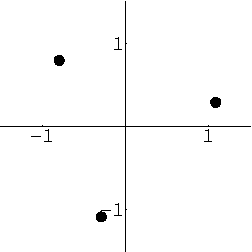
\includegraphics[width=0.3\textwidth]{fcv/number/roots-1i13}
      \end{center}
      \caption{The three roots.}
      \label{roots-1i13}
    \end{figure}
  \item
    \begin{align*}
      \imath^{1/4}
      &= \left( \e^{\imath \pi/2} \right)^{1/4}
      \\
      &= \e^{\imath \pi/8} 1^{1/4}
      \\
      &= \e^{\imath \pi/8} \e^{\imath 2 \pi k/4}, \quad k = 0,1,2,3
      \\
      &= \left\{ \e^{\imath \pi/8}, \e^{\imath 5 \pi/8}, \e^{\imath 9 \pi/8}, \e^{\imath 13 \pi/8} \right\} 
    \end{align*}
    The principal root is
    \[
    \sqrt[4]{\imath} = \e^{\imath \pi/8}.
    \]
    The roots are depicted in Figure~\ref{roots-i14}.
    \begin{figure}[h!]
      \begin{center}
        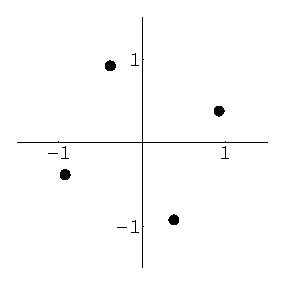
\includegraphics[width=0.3\textwidth]{fcv/number/roots-i14}
      \end{center}
      \caption{The four roots.}
      \label{roots-i14}
    \end{figure}
  \end{enumerate}  
\end{Solution}









\begin{Solution}
  \label{solution Rez+2Imz1}
  \begin{enumerate}
  \item
    \begin{gather*}
      | \Re(z) | + 2 | \Im(z) | \leq 1 \\
      | x | + 2 | y | \leq 1 
    \end{gather*}
    In the first quadrant, this is the triangle below the line 
    $y = (1 - x) / 2$.  We reflect this
    triangle across the coordinate axes to obtain triangles in the 
    other quadrants.  Explicitly, we have the set of points: 
    $\{z = x + \imath y \mid  -1 \leq x \leq 1 \land |y| \leq (1 - |x|) / 2 \}$.
    See Figure~\ref{diamond-112}.
    \begin{figure}[h!]
      \begin{center}
        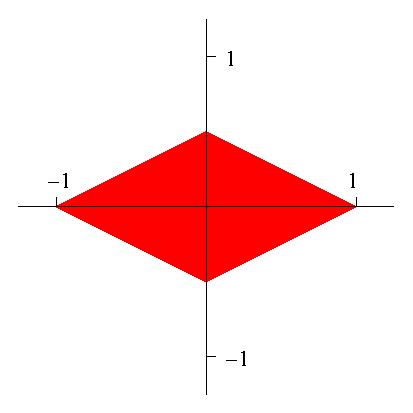
\includegraphics[width=0.3\textwidth]{fcv/number/diamond-112}
      \end{center}
      \caption{The solution is a diamond shape.}
      \label{diamond-112}
    \end{figure}
  \item
    $|z - \imath|$ is the distance from the point $\imath$ in the complex plane.
    Thus $1 < |z - \imath| < 2$ is an annulus centered at $z = \imath$ between the
    radii $1$ and $2$.  See Figure~\ref{annulus-i12}.
    \begin{figure}[h!]
      \begin{center}
        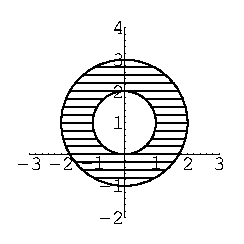
\includegraphics[width=0.25\textwidth]{fcv/number/annulus-i12}
      \end{center}
      \caption{The annulus.}
      \label{annulus-i12}
    \end{figure}
  \item
    The points which are closer to $z = \imath$ than $z = - \imath$ are those points in 
    the upper half plane.  See Figure~\ref{upper-half-domain}.
    \begin{figure}[h!]
      \begin{center}
        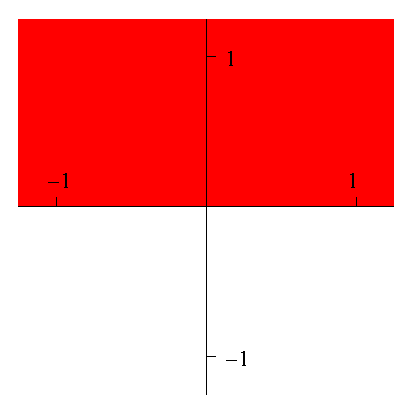
\includegraphics[width=0.3\textwidth]{fcv/number/upper-half-domain}
      \end{center}
      \caption{The upper half plane.}
      \label{upper-half-domain}
    \end{figure}
  \end{enumerate}
\end{Solution}








%% argument identities
\begin{Solution}
  \label{solution argument identities}
  Let $z = r \e^{\imath \theta}$ and $\zeta = \rho \e^{\imath \phi}$.
  \begin{enumerate}
  \item
    \begin{gather*}
      \arg(z \zeta) = \arg(z) + \arg(\zeta) \\
      \arg\left( r \rho \e^{\imath (\theta + \phi)} \right) = \{ \theta + 2 \pi m \} + \{ \phi + 2 \pi n \} \\
      \{ \theta + \phi + 2 \pi k \} = \{ \theta + \phi + 2 \pi m \} 
    \end{gather*}
  \item
    \[
    \Arg(z \zeta) \neq \Arg(z) + \Arg(\zeta)
    \]
    Consider $z = \zeta = -1$.  $\Arg(z) = \Arg(\zeta) = \pi$, however 
    $\Arg(z \zeta) = \Arg(1) = 0$.  The identity becomes $0 \neq 2 \pi$.
  \item
    \begin{gather*}
      \arg\left( z^2 \right) = \arg(z) + \arg(z) \neq 2 \arg(z) 
      \\
      \arg\left( r^2 \e^{\imath 2 \theta} \right) 
      = \{ \theta + 2 \pi k \} + \{ \theta + 2 \pi m \} \neq 2 \{ \theta + 2 \pi n \} 
      \\
      \{ 2 \theta + 2 \pi k \} = \{ 2 \theta + 2 \pi m \} \neq \{ 2 \theta + 4 \pi n \} 
    \end{gather*}
  \end{enumerate}
\end{Solution}





%% triangle inequalities
\begin{Solution}
  \label{solution triangle inequalities}
  Consider a triangle in the complex plane with vertices at $0$, $z$
  and $z + \zeta$.  (See Figure~\ref{triangle}.)
  \begin{figure}[h!]
    \begin{center}
      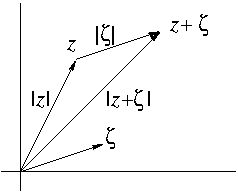
\includegraphics[width=0.3\textwidth]{fcv/number/triangle}
    \end{center}
    \caption{Triangle inequality.}
    \label{triangle}
  \end{figure}

  The lengths of the sides of the triangle are $|z|$, $|\zeta|$ and 
  $|z + \zeta|$  The second inequality shows that one side of the triangle must 
  be less than or equal to the sum of the other two sides.  
  \[
  |z + \zeta| \leq |z| + |\zeta|
  \]
  The first inequality
  shows that the length of one side of the triangle must be greater than
  or equal to the difference in the length of the other two sides.
  \[
  |z + \zeta| \geq ||z| - |\zeta||
  \]

  Now we prove the inequalities algebraically.  We will reduce the inequality
  to an identity.  Let $z = r \e^{\imath \theta}$, $\zeta = \rho \e^{\imath \phi}$.
  \begin{gather*}
    ||z| - |\zeta||\leq |z + \zeta| \leq |z| + |\zeta| 
    \\
    |r - \rho| \leq |r \e^{\imath \theta} + \rho \e^{\imath \phi}| \leq r + \rho 
    \\
    \left( r - \rho \right)^2 \leq \left( r \e^{\imath \theta} + \rho \e^{\imath \phi} \right)
    \left( r \e^{- \imath \theta} + \rho \e^{- \imath \phi} \right) 
    \leq \left( r + \rho \right)^2 
    \\
    r^2 + \rho^2 - 2 r \rho \leq r^2 + \rho^2 + r \rho \e^{\imath \left( \theta - \phi \right)} +
    r \rho \e^{\imath \left( - \theta + \phi \right)} \leq r^2 + \rho^2 + 2 r \rho 
    \\
    - 2 r \rho \leq 2 r \rho \cos\left( \theta - \phi \right) \leq 2 r \rho 
    \\
    -1 \leq \cos(\theta - \phi) \leq 1
  \end{gather*}
\end{Solution}






%% $(-1)^{-3/4}$ $8^{1/6}$
\begin{Solution}
  \label{solution -1 -3/4 8 1/6}
  \begin{enumerate}
    %%
  \item
    \begin{align*}
      (- 1)^{-3/4} 
      &= \left( (- 1)^{-3} \right)^{1/4} 
      \\
      &= (- 1)^{1/4} 
      \\
      &= \left( \e^{\imath \pi} \right)^{1/4} 
      \\
      &= \e^{\imath \pi / 4} 1^{1/4} 
      \\
      &= \e^{\imath \pi / 4} \e^{\imath k \pi / 2}, \quad k = 0,1,2,3 
      \\
      &= \left\{ \e^{\imath \pi / 4}, \e^{\imath 3 \pi / 4}, \e^{\imath 5 \pi / 4}, \e^{\imath 7 \pi / 4} \right\} 
      \\
      &= \left\{ \frac{1 + \imath}{\sqrt{2}}, \frac{- 1 + \imath}{\sqrt{2}},
        \frac{-1 - \imath}{\sqrt{2}}, \frac{1 - \imath}{\sqrt{2}} \right\}
    \end{align*}
    See Figure~\ref{roots_1_3_4}.

    \begin{figure}[h!]
      \begin{center}
        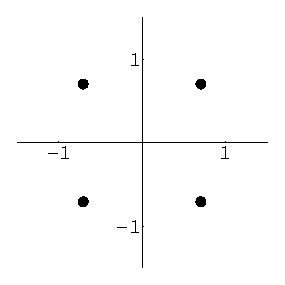
\includegraphics[width=0.3\textwidth]{fcv/number/roots_1_3_4}
      \end{center}
      \caption{The four roots.}
      \label{roots_1_3_4}
    \end{figure}
    %%
  \item
    \begin{align*}
      8^{1/6}
      &= \sqrt[6]{8} 1^{1/6} 
      \\
      &= \sqrt{2} \e^{\imath k \pi / 3}, \quad k = 0,1,2,3,4,5 
      \\
      &= \left\{ \sqrt{2}, 
        \sqrt{2} \e^{\imath \pi / 3},
        \sqrt{2} \e^{\imath 2 \pi / 3},
        \sqrt{2} \e^{\imath \pi},
        \sqrt{2} \e^{\imath 4 \pi / 3},
        \sqrt{2} \e^{\imath 5 \pi / 3} \right\} 
      \\
      &= \left\{ \sqrt{2},
        \frac{1 + \imath \sqrt{3}}{\sqrt{2}},
        \frac{-1 + \imath \sqrt{3}}{\sqrt{2}},
        - \sqrt{2},
        \frac{-1 - \imath \sqrt{3}}{\sqrt{2}},
        \frac{1 - \imath \sqrt{3}}{\sqrt{2}} \right\}
    \end{align*}
    See Figure~\ref{roots_8_1_6}.

    \begin{figure}[h!]
      \begin{center}
        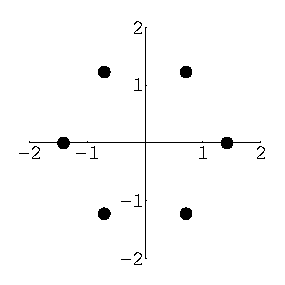
\includegraphics[width=0.3\textwidth]{fcv/number/roots_8_1_6}
      \end{center}
      \caption{The six roots.}
      \label{roots_8_1_6}
    \end{figure}

  \end{enumerate}
\end{Solution}












%% (-1)^{-1/4}
\begin{Solution}
  \label{solution 16 1/8}
  \begin{enumerate}
  \item
    \begin{align*}
      (-1)^{-1/4}
      &= ((-1)^{-1})^{1/4} 
      \\
      &= (-1)^{1/4} 
      \\
      &= \left( \e^{\imath \pi} \right)^{1/4} 
      \\
      &= \e^{\imath \pi / 4} 1^{1/4} 
      \\
      &= \e^{\imath \pi / 4} \e^{\imath k \pi / 2}, \quad k = 0, 1, 2, 3 
      \\
      &= \left\{ \e^{\imath \pi / 4}, \e^{\imath 3 \pi / 4}, \e^{\imath 5 \pi / 4}, \e^{\imath 7 \pi / 4} \right\} 
      \\
      &= \left\{ \frac{1 + \imath}{\sqrt{2}}, \frac{-1 + \imath}{\sqrt{2}},
        \frac{-1 - \imath}{\sqrt{2}}, \frac{1 - \imath}{\sqrt{2}} \right\}
    \end{align*}
    See Figure~\ref{roots_1_1_4}.

    \begin{figure}[h!]
      \begin{center}
        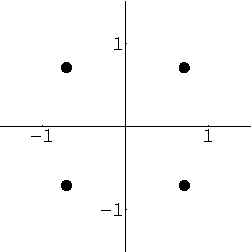
\includegraphics[width=0.3\textwidth]{fcv/number/roots_1_1_4}
      \end{center}
      \caption{The four roots.}
      \label{roots_1_1_4}
    \end{figure}
    %%
  \item
    \begin{align*}
      16^{1/8}
      &= \sqrt[8]{16}  1^{1/8} 
      \\
      &= \sqrt{2} \e^{\imath k \pi / 4}, \quad k = 0,1,2,3,4,5,6,7 
      \\
      &= \left\{ \sqrt{2}, 
        \sqrt{2} \e^{\imath \pi / 4}, 
        \sqrt{2} \e^{\imath \pi / 2}, 
        \sqrt{2} \e^{\imath 3 \pi / 4}, 
        \sqrt{2} \e^{\imath \pi}, 
        \sqrt{2} \e^{\imath 5 \pi / 4}, 
        \sqrt{2} \e^{\imath 3 \pi / 2}, 
        \sqrt{2} \e^{\imath 7 \pi / 4} \right\} 
      \\
      &= \left\{ \sqrt{2}, 
        1 + \imath, 
        \imath \sqrt{2}, 
        - 1 + \imath, 
        - \sqrt{2},
        -1 - \imath, 
        - \imath \sqrt{2}, 
        1 - \imath \right\} 
    \end{align*}
    See Figure~\ref{roots_16_1_8}.

    \begin{figure}[h!]
      \begin{center}
        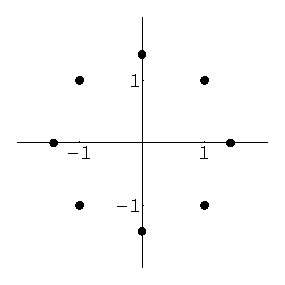
\includegraphics[width=0.3\textwidth]{fcv/number/roots_16_1_8}
      \end{center}
      \caption{The eight roots.}
      \label{roots_16_1_8}
    \end{figure}
  \end{enumerate}
\end{Solution}












%% $1 < |z - 2 \imath| < 2$ $| \Re(z) | + 5 | \Im(z) | = 1$
\begin{Solution}
  \label{solution 1 z-i2 2}
  \begin{enumerate}
    %%
  \item
    $|z - \imath 2|$ is the distance from the point $\imath 2$ in the complex plane.
    Thus $1 < |z - \imath 2| < 2$ is an annulus.  See Figure~\ref{annulus_1_2i}.

    \begin{figure}[h!]
      \begin{center}
        
\includegraphics[width=0.25\textwidth]{fcv/number/annulus_1_2i}
      \end{center}
      \caption{The annulus.}
      \label{annulus_1_2i}
    \end{figure}
    %%
  \item
    \begin{gather*}
      | \Re(z) | + 5 | \Im(z) | = 1 \\
      | x | + 5 | y | = 1 
    \end{gather*}
    In the first quadrant this is the line $y = (1 - x) / 5$.  We reflect this
    line segment across the coordinate axes to obtain line segments in the 
    other quadrants.  Explicitly, we have the set of points: 
    $\{z = x + \imath y \mid -1 < x < 1 \land y = \pm (1 - |x|) / 5 \}$.
    See Figure~\ref{diamond}.

    \begin{figure}[h!]
      \begin{center}
        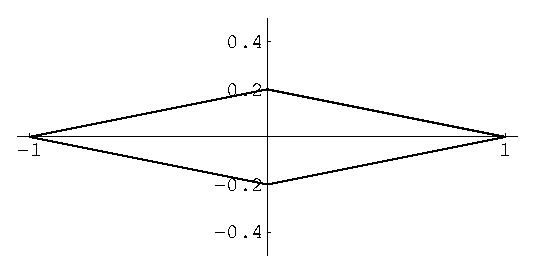
\includegraphics[width=0.5\textwidth]{fcv/number/diamond}
      \end{center}
      \caption{The solution is a diamond shape.}
      \label{diamond}
    \end{figure}
    %%
  \item
    The set of points equidistant from $\imath$ and $-\imath$ is the real axis.
    See Figure~\ref{real_axis}.
    \begin{figure}[h!]
      \begin{center}
        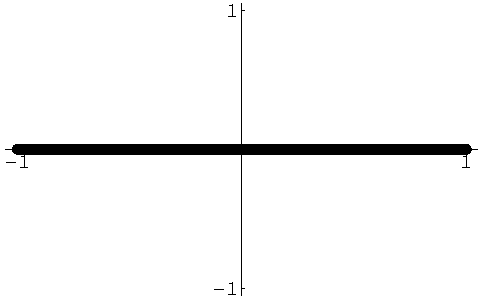
\includegraphics[width=0.4\textwidth]{fcv/number/real_axis}
      \end{center}
      \caption{The solution is the real axis.}
      \label{real_axis}
    \end{figure}
  \end{enumerate}
\end{Solution}















%% |z - 1 + \imath|\leq 1
\begin{Solution}
  \label{solution z-1+i 1}
  \begin{enumerate}
  \item
    $|z - 1 + \imath|$ is the distance from the point $(1 - \imath)$.  Thus 
    $|z - 1 + \imath| \leq 1$ is
    the disk of unit radius centered at $(1 - \imath)$.
    See Figure~\ref{disk_1_mi}.
    \begin{figure}[h!]
      \begin{center}
        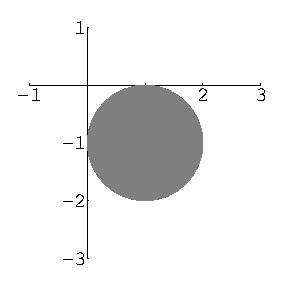
\includegraphics[width=0.3\textwidth]{fcv/number/disk_1_mi}
      \end{center}
      \caption{A disk of unit raduis.}
      \label{disk_1_mi}
    \end{figure}
    %%
  \item
    \begin{gather*}
      \Re(z)- \Im(z) = 5 
      \\
      x - y = 5 
      \\
      y = x - 5
    \end{gather*}
    See Figure~\ref{line_yx5}.
    \begin{figure}[h!]
      \begin{center}
        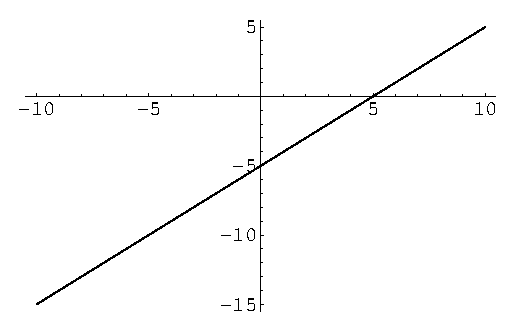
\includegraphics[width=0.5\textwidth]{fcv/number/line_yx5}
      \end{center}
      \caption{The solution is a line.}
      \label{line_yx5}
    \end{figure}
    %%
    %%
    %%
  \item
    Since $|z - \imath| + |z + \imath| \geq 2$, there are no solutions of 
    $|z - \imath| + |z + \imath| = 1$.
  \end{enumerate}
\end{Solution}









%% |\e^{\imath \theta}-1| =2
\begin{Solution}
  \label{solution e i theta - 1 = 2}
  \begin{gather*}
    |\e^{\imath \theta} - 1| = 2 
    \\
    \left( \e^{\imath \theta} - 1 \right) \left( \e^{-\imath \theta} - 1 \right) = 4 
    \\
    1 - \e^{\imath \theta} - \e^{-\imath \theta} + 1 = 4 
    \\
    -2 \cos(\theta) = 2 
    \\
    \theta = \pi
  \end{gather*}

  $\left\{ \e^{\imath \theta} \mid 0 \leq \theta \leq \pi \right\}$ is a unit semi-circle in the
  upper half of the complex plane from $1$ to $-1$.  The only point on this
  semi-circle that is a distance $2$ from the point $1$ is the point $-1$,
  which corresponds to $\theta = \pi$.
\end{Solution}









%%-----------------------------------------------------------------------------
\begin{large}
  \noindent
  \textbf{Polar Form}
\end{large}




%% Euler's formula
\begin{Solution}
  \label{solution eulers formula}
  We recall the Taylor series expansion of $\e^x$ about $x = 0$.
  \[
  \e^x = \sum_{n = 0}^\infty \frac{x^n}{n!}.
  \]
  We take this as the definition of the exponential function for complex
  argument.
  \begin{align*}
    \e^{\imath \theta} 
    &= \sum_{n = 0}^\infty \frac{(\imath \theta)^n}{n!} 
    \\
    &= \sum_{n = 0}^\infty \frac{\imath^n}{n!} \theta^n
    \\
    &= \sum_{n = 0}^\infty \frac{(-1)^n}{(2 n)!} \theta^{2n}
    + \imath \sum_{n = 0}^\infty \frac{(-1)^n}{(2 n + 1)!} \theta^{2n+1}
  \end{align*}
  We compare this expression to the Taylor series for the sine and cosine.
  \[
  \cos \theta = \sum_{n = 0}^\infty \frac{(-1)^n}{(2 n)!} \theta^{2n}, \qquad
  \sin \theta = \sum_{n = 0}^\infty \frac{(-1)^n}{(2 n + 1)!} \theta^{2n+1}, \qquad
  \]
  Thus $\e^{\imath \theta}$ and $\cos \theta + \imath \sin \theta$ have the same Taylor
  series expansions about $\theta = 0$. 
  \[
  \boxed{
    \e^{\imath \theta} = \cos \theta + \imath \sin \theta
    }
  \]
\end{Solution}








%% \cos(3\theta) = \cos^3(\theta) -3\cos(\theta)\sin^2(\theta).
\begin{Solution}
  \label{solution cos 3t = cos3 t - 3 cos t sin2 t}
  \begin{gather*}
    \cos(3 \theta) + \imath \sin(3 \theta) = (\cos \theta + \imath \sin \theta)^3 
    \\
    \cos(3 \theta) + \imath \sin(3 \theta) = \cos^3 \theta + \imath 3 \cos^2 \theta \sin \theta
    - 3 \cos \theta \sin^2 \theta - \imath \sin^3 \theta 
    \\
    \intertext{We equate the real parts of the equation.}
    \cos(3 \theta) = \cos^3 \theta - 3 \cos \theta \sin^2 \theta 
  \end{gather*}
\end{Solution}








%% 1 + z + z^2 + \cdots + z^n = \frac{1 - z^{n+1}}{1-z}, \qquad (z \neq 1),
\begin{Solution}
  \label{solution geometric trig identity}
  Define the partial sum,
  \[
  S_n(z) = \sum_{k=0}^n z^k.
  \]
  Now consider $(1 - z) S_n(z)$.
  \begin{gather*}
    (1 - z) S_n(z) = (1 - z) \sum_{k=0}^n z^k 
    \\
    (1 - z) S_n(z) = \sum_{k=0}^n z^k - \sum_{k=1}^{n+1} z^k 
    \\
    (1 - z) S_n(z) = 1 - z^{n+1} 
    \\
    \intertext{We divide by $1 - z$.  Note that $1 - z$ is nonzero.}
    S_n(z) = \frac{1 - z^{n+1} }{ 1 - z } 
    \\
    1 + z + z^2 + \cdots + z^n = \frac{1 - z^{n+1}}{1 - z}, \qquad (z \neq 1)
  \end{gather*}

  Now consider $z = \e^{\imath \theta}$ where $0 < \theta < 2 \pi$ so that $z$ is not unity.
  \begin{gather*}
    \sum_{k = 0}^n \left( \e^{\imath \theta} \right)^k = \frac{1 - \left( \e^{\imath \theta} \right)^{n+1} }{1 - \e^{\imath \theta}}
    \\
    \sum_{k = 0}^n \e^{\imath k \theta} = \frac{1 - \e^{\imath (n+1) \theta} }{1 - \e^{\imath \theta}} 
    \\
    \intertext{In order to get $\sin(\theta/2)$ in the denominator, we 
      multiply top and bottom by $\e^{-\imath \theta / 2}$.}
    \sum_{k = 0}^n (\cos(k \theta) + \imath \sin(k \theta) ) =
    \frac{\e^{- \imath \theta / 2} - \e^{\imath (n+1/2) \theta} }{\e^{-\imath \theta / 2} - \e^{\imath \theta / 2}} 
    \\
    \sum_{k = 0}^n \cos(k \theta) + \imath \sum_{k = 0}^n \sin(k \theta) =
    \frac{ \cos(\theta/2) - \imath \sin(\theta/2)
      - \cos((n+1/2) \theta) - \imath \sin((n+1/2) \theta) }{ - 2 \imath \sin(\theta/2) } 
    \\
    \sum_{k = 0}^n \cos(k \theta) + \imath \sum_{k = 1}^n \sin(k \theta) =
    \frac{1}{2} + \frac{ \sin((n+1/2) \theta) }{ \sin(\theta/2) }
    + \imath \left( \frac{1}{2} \cot(\theta/2)
      - \frac{ \cos((n+1/2) \theta) }{ \sin(\theta/2) } \right)
  \end{gather*}


  \begin{enumerate}
    %%
  \item
    We take the real and imaginary part of this to obtain the identities.
    \[
    \boxed{
      \sum_{k = 0}^n \cos(k \theta) =
      \frac{1}{2} + \frac{ \sin((n + 1/2) \theta) }
      { 2 \sin(\theta/2) }
      }
    \]
    %%
  \item
    \[
    \boxed{
      \sum_{k = 1}^n \sin(k \theta) =
      \frac{1}{2} \cot(\theta/2) 
      - \frac{ \cos((n+1/2) \theta ) }{ 2 \sin(\theta/2) }
      }
    \]
  \end{enumerate}
\end{Solution}







%%-----------------------------------------------------------------------------
\begin{large}
  \noindent
  \textbf{Arithmetic and Vectors}
\end{large}







%% modulus identities with polar form
\begin{Solution}
  \label{solution modulus identities polar}
  \begin{align*}
    |z \zeta| &= |r \e^{\imath \theta} \rho \e^{\imath \phi} | 
    \\
    &= | r \rho \e^{\imath \left( \theta + \phi \right)} | 
    \\
    &= |r \rho| 
    \\
    &= |r| |\rho| 
    \\
    &= |z| |\zeta|
  \end{align*}
  \begin{align*}
    \left| \frac{z}{\zeta} \right|
    &= \left| \frac{r \e^{\imath \theta}}{\rho \e^{\imath \phi}} \right| 
    \\
    &= \left| \frac{r}{\rho} \e^{\imath \left( \theta - \phi \right)} \right| 
    \\
    &= \left| \frac{r}{\rho} \right| 
    \\
    &= \frac{|r|}{|\rho|} 
    \\
    &= \frac{|z|}{|\zeta|}
  \end{align*}
\end{Solution}









%% parallelogram identity
\begin{Solution}
  \label{solution parallelogram identity}
  \begin{align*}
    \left| z + \zeta \right|^2 + \left| z - \zeta \right|^2
    &= \left( z + \zeta \right) \left( \overline{z} + \overline{\zeta} \right)
    + \left( z - \zeta \right) \left( \overline{z} - \overline{\zeta} \right) 
    \\
    &= z \overline{z} + z \overline{\zeta} + \zeta \overline{z} + \zeta \overline{\zeta}
    + z \overline{z} - z \overline{\zeta} - \zeta \overline{z} + \zeta \overline{\zeta} 
    \\
    &= 2 \left( \left| z \right|^2 + \left| \zeta \right|^2 \right)
  \end{align*}
  Consider the parallelogram defined by the vectors $z$ and $\zeta$.  
  The lengths of the sides are $z$ and $\zeta$ and the lengths of the 
  diagonals are $z + \zeta$ and $z - \zeta$.  
  We know from geometry that the sum of the squared lengths of the diagonals
  of a parallelogram is equal to the sum of the squared lengths of the four
  sides.  (See Figure~\ref{para_identity}.)
  \begin{figure}[h!]
    \begin{center}
      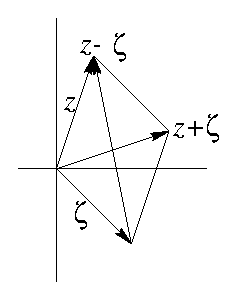
\includegraphics[width=0.15\textwidth]{fcv/number/para_identity}
    \end{center}
    \caption{The parallelogram.}
    \label{para_identity}
  \end{figure}
\end{Solution}



%%-----------------------------------------------------------------------------
\begin{large}
  \noindent
  \textbf{Integer Exponents}
\end{large}



%% (1 + \imath)^{10}
\begin{Solution}
  \label{solution (1+i)10}
  \begin{enumerate}
  \item
    \begin{align*}
      (1 + \imath)^{10}
      &= \left( \left( (1 + \imath)^2 \right)^2 \right)^2 (1 + \imath)^2 
      \\
      &= \left( \left( \imath 2 \right)^2 \right)^2 (\imath 2) 
      \\
      &= \left( -4 \right)^2 (\imath 2) 
      \\
      &= 16 (\imath 2) 
      \\
      &= \imath 32
    \end{align*}
  \item
    \begin{align*}
      (1 + \imath)^{10}
      &= \left( \sqrt{2} \e^{\imath \pi/4} \right)^{10} 
      \\
      &= \left( \sqrt{2} \right)^{10} \e^{\imath 10 \pi/4} 
      \\
      &= 32 \e^{\imath \pi/2} 
      \\
      &= \imath 32
    \end{align*}
  \end{enumerate}
\end{Solution}




%%-----------------------------------------------------------------------------
\begin{large}
  \noindent
  \textbf{Rational Exponents}
\end{large}



%% Quadratic formula
\begin{Solution}
  \label{solution z2 + 2az + b = 0}
  We substitite the numbers into the equation to obtain an identity.
  \begin{gather*}
    z^2 + 2 a z + b = 0 
    \\
    \left( -a + \left( a^2 - b \right)^{1/2} \right)^2 
    + 2 a \left( -a + \left( a^2 - b \right)^{1/2} \right) + b = 0 
    \\
    a^2 -2 a \left( a^2 - b \right)^{1/2} + a^2 - b - 2 a^2 
    + 2 a \left( a^2 - b \right)^{1/2} + b = 0 
    \\
    0 = 0
  \end{gather*}
\end{Solution}









\raggedbottom

}
